\chapter{Numerik von Hamilton-Systemen}

\section{Hamilton-Systeme}

Extrem wichtige Klasse von Differentialgleichungen entstammen der klassischen Mechanik, Quantenmechanik und relativistische Mechanik. Dazu gehören auch spezielle numerische Verfahren --- eine \enquote{schöne Mathematik}.

\enquote{Vereinigendes Prinzip}: Bringt ganz unterschiedliche Gleichungen auf eine gemeinsame Form.


\begin{bsp}
	Mathematisches Pendel -- Fadenpendel
	\begin{itemize}
		\item Koordinate: Winkel $\alpha$
		\item Masse $m$, Fadenlänge $l$, Erdbeschleunigung $g$
	\end{itemize}
	Bewegungsgleichungen: $\displaystyle \ddot \alpha + \frac{g}{l} \sin \alpha = 0$
\end{bsp}

\begin{bsp}
	Teilchen in einem Kraftfeld $F(x)$
	\begin{equation}
	m \ddot x = F(x) \tag{Newtons Gesetz}
	\end{equation}
\end{bsp}

\begin{bsp}
	1d-Wellengleichung --- Longitudinale Auslenkung einer elastischen Schnur
	\begin{alignat*}{2}
	\frac{\partial^2 u}{\partial x^2} & = \frac{\partial^2 u}{\partial t^2} & \qquad & x \in [a, b], t \ge 0 \\
	u(a, t) = u(b, t) & = 0 && \forall t \ge 0
	\end{alignat*}
\end{bsp}


\subsection{Die Lagrange-Gleichungen}
\label{sec:lagrange_gleichung}

Wir betrachten ein mechanisches System mit $d$ Freiheitsgraden $q = (q_1, \dots, q_d)$.
\begin{itemize}
	\item Kinetische Energie: $T = T(q, \dot q)$
	(häufig: $T(q, \dot{q}) = \frac12 \dot{q}^T M(q) \dot{q}$ mit $M(q)$ s.p.d.)
	\item Potentielle Energie: $U = U(q)$
\end{itemize}

\begin{definition}
	Die Lagrange-Funktion eines mechanischen Systems ist $L = T - U$.
\end{definition}

Das mechanische System löst die Lagrange-Gleichungen
\begin{equation*}
\frac{d}{dt} \left( \frac{\partial L}{\partial \dot q} \right) = \frac{\partial L}{\partial q}
\end{equation*}

\emph{Warum?} Es gilt das Prinzip der stationären Wirkung.

\begin{definition}[Prinzip der stationären Wirkung / Hamilton'sches Prinzip]
	Sei $q: [t_0, t_1] \to \R^d$ eine Trajektorie eines mechanischen Systems.
	Für die in der Natur vorkommenden Trajektorien ist die \textit{Wirkung}
	\begin{equation*}
	W \colonequals \int_{t_0}^{t_1} L(q(t) \ \dot q(t)) \dt
	\end{equation*}
	stationär.
\end{definition}

Sei $q$ eine Trajektorie, und $\delta q$ eine Variation davon, die die Endpunkte fest lässt, also $\delta q(t_0)=\delta q(t_1) = 0$.
Stationarität von $q$ heißt dann, dass für alle solche $\delta q$
\begin{equation*}
\frac{d}{d\epsilon} S(q+\epsilon\delta q)\vert_{\epsilon=0} = 0.
\end{equation*}
gilt. Ausrechnen:
\begin{align*}
\frac{d}{d\epsilon} \int_{t_0}^{t_1} L(q+ \epsilon\delta q,\dot q + \epsilon\delta \dot q)\dt\vert_{\epsilon=0} &= \int_{t_0}^{t_1} \frac{\partial L}{\partial q}\delta q + \frac{\partial L}{\partial\dot q} \delta\dot q\, dt \\
&= \int_{t_0}^{t_1} \Bigg(\frac{\partial L}{\partial q} \delta q - \frac{d}{dt} \frac{\partial L}{\partial \dot q} \delta q\Bigg)\dt \tag{partielle Integration} \\
&= \int_{t_0}^{t_1} \Bigg(\frac{\partial L}{\partial q} - \frac{d}{dt} \frac{\partial L}{\partial \dot q}  \Bigg)\delta q\dt
\end{align*}
Da dieser Ausdruck für alle hinreichend glatten Funktionen $\delta q$ gleich Null sein muss, erhält man die Lagrange-Gleichung
\begin{equation*}
\delta W = 0 = \frac{d}{dt} \left( \frac{\partial L}{\partial \dot q} \right) - \frac{\partial L}{\partial q}
\end{equation*}

\begin{bsp}[Pendel]
	\begin{itemize}
		\item Kinetische Energie
		\begin{equation*}
		T = \frac12 m (\dot x^2 + \dot y^2) = \frac12 m l^2 \dot\alpha^2
		\end{equation*}
		\item Potentielle Energie
		\begin{equation*}
		U = mgy = -mgl \cos \alpha
		\end{equation*}
		\item Lagrange-Funktion
		\begin{equation*}
		L(\alpha, \dot\alpha) = \frac12 m l^2 \dot\alpha^2 + mgl \cos \alpha
		\end{equation*}
		\item Lagrange-Gleichung
		\begin{equation*}
		0
		= \frac{d}{dt} \left( \frac{\partial L}{\partial \dot q} \right) - \frac{\partial L}{\partial q}
		= \frac{d}{dt}( ml^2\dot\alpha ) + mgl \sin \alpha
		= ml^2\ddot\alpha + mgl \sin \alpha.
		\end{equation*}
	\end{itemize}
\end{bsp}

\begin{bsp}[Teilchen in einem Kraftfeld]
	Angenommen das Kraftfeld ist \emph{konservativ}, d.h. es gibt ein $U: \R^3 \to \R$, so dass $F(x) = -\nabla U(x)$.
	\begin{itemize}
		\item Kinetische Energie
		\begin{equation*}
		T(x, \dot x) = \frac12 m \langle \dot x, \dot x \rangle
		\end{equation*}
		\item Potentielle Energie
		\begin{equation*}
		U
		\end{equation*}
		\item Lagrange-Gleichung
		\begin{equation*}
		0
		= \frac{d}{dt} \left( \frac{\partial L}{\partial \dot q} \right) - \frac{\partial L}{\partial q}
		= \frac{d}{dt}(m\dot x) + \nabla U(x) = m\ddot x - F(x)
		\end{equation*}
	\end{itemize}
\end{bsp}

\begin{bsp}[Eindimensionale Wellengleichung]
	Ein unendlich-dimensionales System wird nicht beschrieben durch $d$
	Freiheitsgrade $(q_1, \dots, q_d)$, sondern durch die Funktion $u: [a, b] \to \R$. Diese beschreibt die transversale Auslenkung einer Saite.
	\begin{itemize}
		\item Kinetische Energie
		\begin{equation*}
		T(u, \dot u) = \frac12 \int_a^b m \dot u(x)^2 dx
		\end{equation*}
		Dabei ist $m$ die Massendichte.
		\item Potentielle Energie
		\begin{equation*}
		U(u)
		=
		\int_a^b S \Big[ \sqrt{1+ u'(x)^2} -1 \Big] dx
		\approx
		\int_a^b S\frac{u'(x)^2}{2} dx
		\end{equation*}
		Dabei ist $S$ die Zugsteifigkeit.
		\item Lagrange-Funktion
		\begin{equation*}
		L(u, \dot u) = T(u, \dot u) - U(u)
		\end{equation*}
		\item Lagrange-Gleichung
		\begin{equation*}
		\frac{\partial L}{\partial u}
		=
		\frac{\partial}{\partial x} \frac{\partial L}{\partial u'}
		+ \frac{\partial}{\partial t} \frac{\partial L}{\partial \dot{u}}
		\end{equation*}
		Einsetzen:
		\begin{equation*}
		0 =
		\frac{\partial}{\partial x} \Big(- S u'(x)\Big)
		+ \frac{\partial}{\partial t}m\dot{u}
		\end{equation*}
		Umstellen:
		\begin{equation*}
		\frac{\partial^2 u}{\partial t^2} = \frac{S}{m} \frac{\partial^2 u}{\partial x^2}
		\end{equation*}
		Das ist die eindimensionale Wellengleichung.
	\end{itemize}
\end{bsp}


%\subsection{Die Hamiltonschen Gleichungen}
%
%Eine Transformation der Lagrange-Gleichung;
%quasi \glqq die andere Seite der Medaille\grqq
%
%\begin{itemize}
%\item Definiere die Impulse
%  \begin{equation*}
%    p_k \colonequals \frac{\partial L}{\partial \dot q_k}(q, \dot q) \qquad \text{für } k = 1, \dots, d
%  \end{equation*}
%  Diese Abbildung heißt \emph{Legendre-Transformation}.
%\end{itemize}
%
%\begin{definition}
%  Die Hamilton-Funktion ist
%  \begin{equation*}
%    H(p, q) \colonequals p^T \dot q - L(q, \dot q).
%  \end{equation*}
%\end{definition}
%
%Dabei geht man natürlich davon aus, dass die Legendre-Transformation eine $C^1$-Bijektion $\dot q \leftrightarrow p$ darstellt.
%
%\emph{Beispiel}: kinetische Energie ist quadratisch:
%
%\begin{equation*}
%  T = \frac 12 \dot q^T M \dot q \qquad \text{ mit $M$ s.p.d.}
%\end{equation*}
%
%\begin{itemize}
%\item Legendre-Transformation: Für festes $q$ hat man
%  \begin{equation*}
%    p = M \dot q.
%  \end{equation*}
%  Transformation ist also tatsächlich glatte Bijektion.
%\item Hamilton-Funktion
%  \begin{align*}
%    H(p, q)
%    & = p^T \dot q - L(q, \dot q) \\
%    & = p^T M^{-1} p - L(q, M^{-1} p) \\
%    & = p^T M^{-1} p - T(q, M^{-1} p) + U(q) \\
%    & = p^T M^{-1} p - \frac12 (M^{-1}p)^T M (M^{-1} p) + U(q) \\
%    & = \frac12 (M^{-1}p)^T M (M^{-1}p) + U(q) \\
%    & = T + U
%  \end{align*}
%  Die Hamilton-Funktion ist die Gesamtenergie!
%\end{itemize}
%
%Auch mit Hilfe der Hamilton-Funktion kann man das Verhalten des mechanischen Systems einfach ausdrücken.
%
%\begin{satz}[{\citet[Thm.\,VI.1.3]{hairer_lubich_wanner:2006}}]
%  Die Lagrange-Gleichung ist äquivalent zu den Hamilton-Gleichungen
%  \begin{equation*}
%    \dot p_k = -\frac{\partial H}{\partial q_k}(p, q),
%    \quad
%    \dot q_k = \frac{\partial H}{\partial p_k}(p, q),
%    \qquad
%    k = 1, \dots, d.
%  \end{equation*}
%\end{satz}
%
%\begin{proof}
%  Lagrange $\implies$ Hamilton (die andere Richtung ist ähnlich)
%  \begin{align*}
%    \frac{\partial H}{\partial q}
%    & = \frac\partial{\partial q}\left( p^T \dot q - L(q, \dot q) \right) & \text{(Def. von $H$)} \\
%    & = p^T \frac{\partial \dot q}{\partial q} - \frac{\partial L}{\partial q} - \underbrace{\frac{\partial L}{\partial \dot q}}_{= p^T} \frac{\partial \dot q}{\partial q} & \text{(Kettenregel)} \\
%    & = - \frac{\partial L}{\partial q} & \text{(Def. von $p = \frac{\partial L}{\partial \dot q}$)} \\
%    & = - \frac{d}{dt}\left( \frac{\partial L}{\partial \dot q} \right) & \text{(Lagrange-Gleichung)} \\
%    & = - \dot p & \text{(Def. von $p$)}
%  \end{align*}
%  Und:
%  \begin{align*}
%    \frac{\partial H}{\partial p}
%    & = \frac{\partial}{\partial p}\left( p^T \dot q - L(q, \dot q) \right) \\
%    & = \dot q + p^T \frac{\partial \dot q}{\partial p} - \underbrace{\frac{\partial L}{\partial \dot q}}_{=p^T} \frac{\partial \dot q}{\partial p} & \text{(Produktregel; $q$ hängt nicht von $p$ ab)} \\
%    & = \dot q \qedhere
%  \end{align*}
%\end{proof}
%
%Sowohl die Lagrangesche als auch die Hamiltonsche Formulierungen haben ihre Daseinsberechtigung.
%\begin{itemize}
%\item Die Lagrange-Formulierung ist besonders fundamental: sie beruht auf Variationsprinzipien
%\item Die Hamilton-Formulierung ist besonders fundamental: sie beruht auf der Gesamtenergie des Systems.
%\end{itemize}
%
%\emph{Beispiel}: Pendel (mit $q = \alpha$)
%\begin{itemize}
%\item Kinetische Energie
%  \begin{equation*}
%    T = \frac12 m l^2 \dot q^2
%  \end{equation*}
%\item Potentielle Energie
%  \begin{equation*}
%    U = -mgl \cos q
%  \end{equation*}
%
%\item Impuls
%  \begin{equation*}
%    p
%    \colonequals \frac{\partial L}{\partial\dot q}
%    = \frac{\partial}{\partial\dot q}\Big( \frac12 m l^2 \dot q^2 + mgl \cos q \Big)
%    = m l^2 \dot q
%  \end{equation*}
%\item Kinetische Energie ist quadratisch, also
%  \begin{align*}
%    H(p, q)
%    & = T(p, q) + U(q) \\
%    & = \frac12 m l^2 \dot q^2 - m g l \cos q \\
%    & = \frac12 \frac{1}{m l^2} p^2 - m g l \cos q
%  \end{align*}
%\item Bewegungsgleichungen:
%  \begin{eqnarray*}
%    \dot p = -\frac{\partial H}{\partial q} & \Leftrightarrow & \dot p = - m g l \sin q \\
%    \dot q = \frac{\partial H}{\partial p} & \Leftrightarrow & \dot q = \frac{1}{m l^2} p
%  \end{eqnarray*}
%\end{itemize}
%
%In der letzten Vorlesung hatten wir gesehen, dass das Pendel die Größe
%\begin{equation*}
%  \frac12 \frac{1}{ml^2} p^2 - mgl \cos q = T(p, q) + U(p)
%\end{equation*}
%erhält.
%Das ist kein Zufall.
%
%\begin{satz}
%  Die Hamilton-Funktion $H$ ist Invariante des Flusses der Hamiltonschen Gleichung.
%\end{satz}
%
%\begin{proof}
%  \begin{align*}
%    \frac{d}{dt} H(p, q)
%    & = \frac{\partial H}{\partial p} \dot p + \frac{\partial H}{\partial q} \dot q & \text{(Kettenregel)} \\
%    & = \frac{\partial H}{\partial p} \Big(-\frac{\partial H}{\partial q}\Big)
%      + \frac{\partial H}{\partial q} \Big(\frac{\partial H}{\partial p}\Big) & \text{(Hamiltonsche Gl.)} \\
%    & = 0 \qedhere
%  \end{align*}
%\end{proof}
%
%Diese sehr allgemeine Erhaltungseigenschaft wollen wir natürlich ins Diskrete übertragen!

\section{Symplektizität}

Flüsse von Hamiltonschen Systemen haben eine weitere wichtige Erhaltungseigenschaft, die sogenannte \begriff{Symplektizität}, die ähnlich wie Volumenerhaltung im Phasenraum vorstellbar ist.

\begin{bsp}
	Volumenerhaltung beim mathematischen Pendel (Bild aus \cite{hairer_lubich_wanner:2006}):
	\begin{center}
		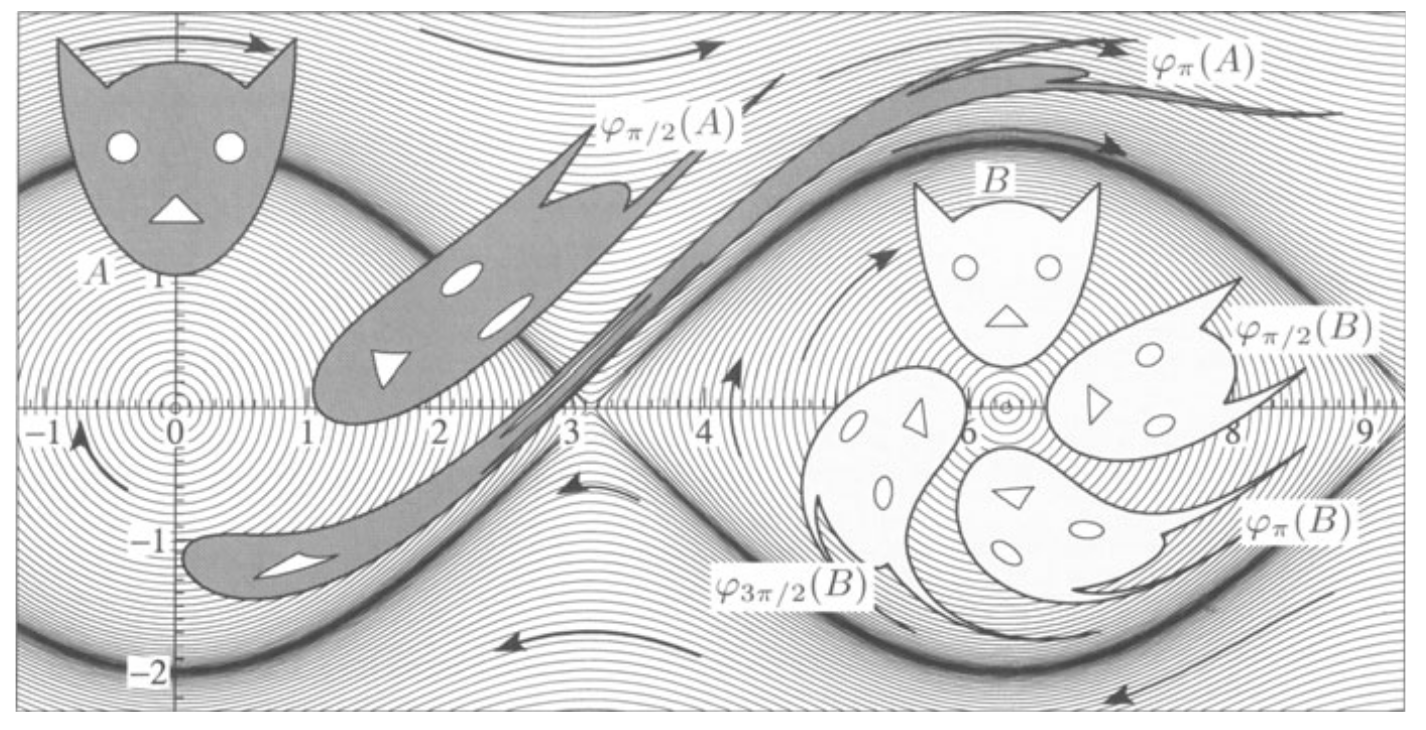
\includegraphics[width=0.8\textwidth]{pendulum-symplecticity-cats}
	\end{center}
\end{bsp}



Betrachte die Hamiltonschen Gleichungen
\begin{equation*}
	\dot p = - \frac{\partial H}{\partial q}(p, q),
	\quad
	\dot q = \frac{\partial H}{\partial p}(p, q)
\end{equation*}

Umschreiben:
\begin{equation*}
	\begin{pmatrix} \dot p \\ \dot q \end{pmatrix}
	=
	\begin{pmatrix} 0 & I \\ -I & 0 \end{pmatrix}^{-1}
	\begin{pmatrix} \frac{\partial H}{\partial p} \\ \frac{\partial H}{\partial q} \end{pmatrix}
\end{equation*}

Diese Beziehung wollen wir jetzt abstrakter betrachten.

\begin{bem}
	Die harmlos aussehende Matrix $\left(\begin{smallmatrix} 0 & I \\ -I & 0 \end{smallmatrix}\right)$ hat eine besondere Eigenschaft.
	Es gilt nämlich
	\begin{equation*}
		\begin{pmatrix} 0 & I \\ -I & 0 \end{pmatrix}^2
		= - \begin{pmatrix} I & 0 \\ 0 & I \end{pmatrix}.
	\end{equation*}
	Sie verhält sich also wie die imaginäre Einheit $i$ und erzeugt damit eine komplexe Struktur auf $\R^{2d}$.
\end{bem}

Wir betrachten $2$-dimensionale Parallelogramme in $\R^{2d}$ aufgespannt durch Vektoren
\begin{equation*}
	\xi = \begin{pmatrix} \xi^p \\ \xi^q \end{pmatrix},
	\quad
	\eta = \begin{pmatrix} \eta^p \\ \eta^q \end{pmatrix}.
\end{equation*}
Hier und im Folgenden bezeichnen $\xi^p \in \R^d$ und $\xi^q \in \R^d$ die Impuls- bzw.\ Ortskomponenten
von $\xi$.

Falls $d = 1$, so ist die orientierte Fläche des Parallelogramms gerade
\begin{equation*}
	\det\begin{pmatrix} \xi^p & \eta^p \\ \xi^q & \eta^q \end{pmatrix}
	= \xi^p \eta^q - \xi^q \eta^p
	= (\xi^p \quad \xi^q)
	\begin{pmatrix} 0 & 1 \\ -1 & 0 \end{pmatrix}
	\begin{pmatrix} \eta^p \\ \eta^q \end{pmatrix}.
\end{equation*}

Das verallgemeinern wir jetzt für höhere Dimensionen.

\begin{definition}[Symplektische Form]
	Die symplektische Form $\omega: \R^{2d} \times \R^{2d} \to \R$ ist
	\begin{equation*}
		\omega(\xi, \eta)
		\colonequals \sum_{i=1}^d \det\begin{pmatrix} \xi_i^p & \eta_i^p \\ \xi_i^q & \eta_i^q \end{pmatrix}
		= \sum_{i=1}^d \left( \xi_i^p \eta_i^q - \xi_i^q \eta_i^p \right).
	\end{equation*}
\end{definition}

\begin{itemize}
	\item Bilineare Form
	\item Interpretation: Summe der orientierten Flächen der Projektionen auf die Koordinatenebenen $(p_i, q_i)$.
	\item Matrixdarstellung
	\begin{equation*}
		\omega(\xi, \eta) =
		\begin{pmatrix} {\xi^p}^T & {\xi^q}^T \end{pmatrix}
		\begin{pmatrix} 0 & I \\ -I & 0 \end{pmatrix}
		\begin{pmatrix} \eta^p \\ \eta^q \end{pmatrix}.
	\end{equation*}
\end{itemize}

Da die Matrix $\begin{pmatrix} 0 & I \\ -I & 0 \end{pmatrix}$ wichtig zu sein scheint geben wir ihr den Namen $J$.

Eine wichtige Eigenschaft von Hamiltonschen Systemen ist nun, dass ihre Flüsse $\Phi^t \colon \R^{2d} \to \R^{2d}$ die symplektische Form erhalten. Das muss man natürlich erklären.

\begin{definition}[Lineare symplektische Abbildung]
	Eine lineare Abbildung $A: \R^{2d} \to \R^{2d}$ heißt \emph{symplektisch}, wenn
	\begin{equation*}
		\omega(A\xi, A\eta) = \omega(\xi, \eta) \qquad \forall \xi, \eta \in \R^{2d}.
	\end{equation*}
	Alternativ: wenn $A^T J A = J$.
\end{definition}

\begin{bem}
	Für $d=1$ bedeutet das gerade, dass $A$ flächenerhaltend ist.
\end{bem}

\begin{definition}[Differenzierbare symplektische Abbildung]
	Sei $U$ eine offene Teilmenge von $\R^{2d}$.
	Eine differenzierbare Abbildung $g: U \to \R^{2d}$ heißt \begriff{symplektisch}, falls die Jacobi-Matrix $\nabla g(p,q)$ für alle $(p, q) \in U$ symplektisch ist.
\end{definition}

Jetzt kommt der zentrale Satz: die Flüsse $\Phi^t$ von Hamiltonschen Systemen erhalten die symplektische Form:

\begin{satz}[Poincaré, 1899]
	Sei $H(p, q)$ zweimal stetig differenzierbar auf $U \subset \R^{2d}$.
	Sei $\Phi^t$ der Phasenfluss der Differentialgleichung
	\begin{equation*}
		\dot y = J^{-1} \nabla H(y)
	\end{equation*}
	mit $y = (p, q)$.

	Für jedes feste $t$ ist $\Phi^t$ eine symplektische Abbildung.
\end{satz}

\begin{proof}
	Der Beweis erfolgt in zwei Schritten:
	\begin{enumerate}
		\item $\Phi^0$ ist symplektisch.
		\item Die \enquote{Abweichung von der Symplektizität} hängt nicht von $t$ ab.
	\end{enumerate}
	
	\begin{enumerate}[label=(zu \arabic*), leftmargin=*]
		\item $\Phi^0$ ist symplektisch, wenn seine erste Ableitung an jedem Punkt $y_0 = (p_0, q_0)$ symplektisch ist. Da $\Phi^0 y_0 = y_0$ gilt
		\begin{equation*}
			\left( \frac{\partial \Phi^0 y_0}{\partial y_0} \right)^T J \left( \frac{\partial \Phi^0 y_0}{\partial y_0} \right)
			= I^T J I
			= J
		\end{equation*}
		Also ist $\Phi^0$ symplektisch.
		
		\item Wir müssen die Ableitung $\frac{\partial \Phi^t y_0}{\partial y_0}$ untersuchen, d.h. die linearisierte Störung der Lösung bei einer Störung des Startwerts -- also gerade die Wronski-Matrix $\Xi$. Diese löst die Gleichung
		\begin{equation*}
			\dot \Xi = J^{-1} \underbrace{\nabla^2 H( \Phi^t(y_0) )}_{\text{Hesse-Matrix von $H$}} \Xi
		\end{equation*}
		Konkret heißt das hier
		\begin{equation}
			\label{eq:wronski_symplectic_form}
			\frac{d}{dt} \frac{\partial \Phi^t}{\partial y_0}
			= J^{-1} \nabla^2 H(\Phi^t y_0) \frac{\partial \Phi^t}{\partial y_0}
		\end{equation}
		Die Produktregel liefert uns
		\begin{equation*}
			\frac{d}{dt}\bigg[ \bigg(\frac{\partial \Phi^t}{\partial y_0}\bigg)^T J \bigg(\frac{\partial \Phi^t}{\partial y_0}\bigg) \bigg]
			= \bigg( \frac{d}{dt} \frac{\partial \Phi^t}{\partial y_0} \bigg)^T J \bigg( \frac{\partial \Phi^t}{\partial y_0} \bigg)
			+ \bigg( \frac{\partial \Phi^t}{\partial y_0} \bigg)^T J \bigg( \frac{d}{dt} \frac{\partial \Phi^t}{\partial y_0} \bigg)
		\end{equation*}
		Dort wird jetzt \eqref{eq:wronski_symplectic_form} eingesetzt:
		\begin{equation*}
			\frac{d}{dt}\bigg[ \bigg(\frac{\partial \Phi^t}{\partial y_0}\bigg)^T J \bigg(\frac{\partial \Phi^t}{\partial y_0}\bigg) \bigg]
			=
			\bigg(\frac{\partial \Phi^t}{\partial y_0}\bigg)^T \nabla^2 H(\Phi^t y_0)^T J^{-T} J \bigg(\frac{\partial \Phi^t}{\partial y_0}\bigg)
			+ \bigg(\frac{\partial \Phi^t}{\partial y_0}\bigg)^T J J^{-1} \nabla^2 H(\Phi^t y_0) \bigg(\frac{\partial \Phi^t}{\partial y_0}\bigg)
		\end{equation*}
		Aber $J^T = -J$, also $J^{-T} J = -I$, und $\nabla^2 H$ ist symmetrisch. Deshalb ist
		\begin{equation*}
			\frac{d}{dt}\bigg[ \bigg(\frac{\partial \Phi^t}{\partial y_0}\bigg)^T
			J
			\bigg(\frac{\partial \Phi^t}{\partial y_0}\bigg) \bigg]
			= 0
		\end{equation*}
	\end{enumerate}
\end{proof}

Es gilt sogar die Umkehrung des Satzes:
\textit{nur} Hamiltonsche Systeme haben symplektische Flüsse!

\begin{definition}[lokal Hamiltonsch]
	Eine Differentialgleichung $x' = f(x)$ heißt \begriff{lokal Hamiltonsch}, wenn für jedes $x_0 \in U$ eine Umgebung existiert, in der
	\begin{equation*}
		f(x) = J^{-1} \nabla H(x)
	\end{equation*}
	für eine Funktion $H$.
\end{definition}

\begin{satz}[{{{\cite[Satz~VI.2.6]{hairer_lubich_wanner:2006}}}}]
	Sei $f \colon U \to \R^{2d}$ stetig differenzierbar.
	Dann ist $x' = f(x)$ genau dann lokal Hamiltonsch, wenn der Fluss $\Phi^t x$ für alle $x \in U$ und alle $t$ hinreichend klein symplektisch ist.
\end{satz}




\section{Symplektische Verfahren}

Wir wollen Verfahren entwickeln, die die Symplektizität von Hamiltonschen Flüssen erben.

\begin{definition}
	Ein Einschrittverfahren heißt symplektisch, falls der diskrete Fluss
	\begin{equation*}
		\Psi^t \colon \R^{2d}\to\R^{2d}
	\end{equation*}
	symplektisch ist, wenn das Verfahren auf ein Hamiltonsches System angewendet wird.
\end{definition}

Die einfachsten symplektischen Verfahren sind die symplektischen Euler-Verfahren
\begin{align*}
	p_{k+1} &= p_k - \tau H_q(p_{k+1},q_k) \\
	q_{k+1} &= q_k + \tau H_p(p_{k+1},q_k)
\end{align*}
und
\begin{align*}
	p_{k+1} &= p_k - \tau H_q(p_k,q_{k+1}) \\
	q_{k+1} &= q_k + \tau H_p(p_k,q_{k+1}).
\end{align*}

\begin{satz}[{{\cite[Satz~VI.3.3]{hairer_lubich_wanner:2006}}}]
	Die symplektischen Euler-Verfahren sind symplektisch.
\end{satz}
\begin{proof}
	Beweis für die erste Methode:
	\begin{itemize}
		\item Methode ist symplektisch, wenn
		\begin{equation*}
		\frac{\partial\Psi^\tau y}{\partial y}\in \R^{2d\times 2d}
		\end{equation*}
		für alle $y=(p,q)$ die symplektisch Form erhält, wenn also
		\begin{equation}\label{eq:symplektische_form}
		\Big(\frac{\partial\Psi^\tau y}{\partial y}\Big)^TJ\Big(\frac{\partial\Psi^\tau y}{\partial y}\Big) = J.
		\end{equation}
		\item Wir bestimmen die vier Komponenten von $\frac{\partial\Psi^\tau y}{\partial y}$:
		\item [1)] Erste Gleichung des Verfahrens:
		\begin{equation*}
		p_{k+1} = p_k - \tau H_q(p_{k+1},q_k)
		\end{equation*}
		Ableiten nach $p_k$:
		\begin{equation*}
		\frac{\partial p_{k+1}}{\partial p_k} = I - \tau H_{qp}(p_{k+1},q_k)\cdot \frac{\partial p_{k+1}}{\partial p_k}
		\end{equation*}
		$\Leftrightarrow$
		\begin{equation*}
		\frac{\partial p_{k+1}}{\partial p_k}\Big(I + \tau H_{qp}\Big) = I
		\end{equation*}
		Ebenso z.B.
		\begin{equation*}
		\frac{\partial p_{k+1}}{\partial q_k}\Big(I + \tau H_{qp}\Big) = -\tau H_{qq}
		\end{equation*}
		etc.
	\end{itemize}
	Zusammen erhält man
	\begin{equation*}
	\begin{pmatrix}
	I + \tau H_{qp}^T & 0 \\ -\tau H_{pp} & I
	\end{pmatrix}
	\begin{pmatrix}
	\frac{\partial p_{k+1}}{\partial p_k} & 	\frac{\partial p_{k+1}}{\partial q_k} \\
	\frac{\partial q_{k+1}}{\partial p_k}  & 	\frac{\partial q_{k+1}}{\partial q_k}
	\end{pmatrix}
	=
	\begin{pmatrix}
	I & -\tau H_{qq} \\ 0 & I+\tau H_{qp}
	\end{pmatrix},
	\end{equation*}
	also
	\begin{equation*}
	\frac{\partial \Psi^\tau y}{\partial y} = \begin{pmatrix}
	I + \tau H_{qp}^T & 0 \\ -\tau H_{pp} & I
	\end{pmatrix}^{-1} \begin{pmatrix}
	I & -\tau H_{qq} \\ 0 & I+\tau H_{qp}
	\end{pmatrix}.
	\end{equation*}
	Damit kann man die Erhaltungseigenschaft \eqref{eq:symplektische_form} direkt nachrechnen.
\end{proof}

Die symplektischen Euler-Verfahren sind \emph{keine} RK-Verfahren. 
Stattdessen gehören sie zu den sog.\ \emph{partitionierten} RK-Verfahren.
Betrachte Differentialgleichungen der Form
\begin{equation*}
	y'=f(y,z),\qquad z'=g(y,z),
\end{equation*}
wobei $y\in\R^{n_1}$ und $z\in\R^{n_2}$. 

\textbf{Idee:} Nimm für $y$ und $z$ zwei verschiedene RK-Verfahren.
Details bei \cite[Kapitel II.2]{hairer_lubich_wanner:2006}

Es gibt auch ein \enquote{einfaches} Verfahren zweiter Ordnung, das symplektisch ist.
\begin{satz}[{{\cite[Satz~VI.3.5]{hairer_lubich_wanner:2006}}}]
	Die implizite Mittelpunktsregel
	\begin{equation*}
		y_{k+1} = y_k + \tau J^{-1}\nabla H\Big( \frac{y_{k+1}+y_k}{2}\Big)
	\end{equation*}
	ist symplektisch.
\end{satz}
\begin{proof}
	Wir leiten wieder ab
	\begin{align*}
		\frac{\partial \Psi^\tau y_k}{\partial y_k} &= \frac{\partial y_{k+1}}{\partial y_k} \\
		&= I + \tau J^{-1} \nabla^2 H\Big( \frac{y_{k+1} + y_k}{2} \Big) \cdot \Big( \frac{1}{2} \frac{\partial y_{k+1}}{y_k} + \frac{1}{2}\Big).
	\end{align*}
	Umformen ergibt
	\begin{align*}
		\frac{\partial y_{k+1}}{\partial y_k}
		&= \Big( I - \frac{\tau}{2} J^{-1}\nabla^2H\Big)^{-1}\Big(I+\frac{\tau}{2}J^{-1}\nabla^2 H\Big).
	\end{align*}
	Dann kann man direkt nachrechnen dass
	$\Big(\frac{\partial y_{k+1}}{\partial y_k}\Big)^T J \frac{\partial y_{k+1}}{\partial y_k} = J$.

	\todoannot{1.5\baselineskip}{Ein paar Details zu dieser Rechnung einfügen!}
\end{proof}


\subsection{Symplektische RK-Verfahren}

Dabei handelt es sich um relativ neue Verfahren, die erst Ende der 1980er Jahre systematisch untersucht wurden.

Wir interessieren uns wieder für die Ableitung
\begin{equation*}
	\Xi(t) = \frac{\partial \Phi^t y_0}{\partial y_0}.
\end{equation*}
Diese löst bekanntlich eine lineare Differentialgleichung.

\begin{lemma}[{{\cite[Lemma VI.4.1]{hairer_lubich_wanner:2006}}}]
	Das folgende Diagramm kommutiert für alle Runge-Kutta-Verfahren und alle partitionierten Runge-Kutta-Verfahren:\\
	\begin{center}
		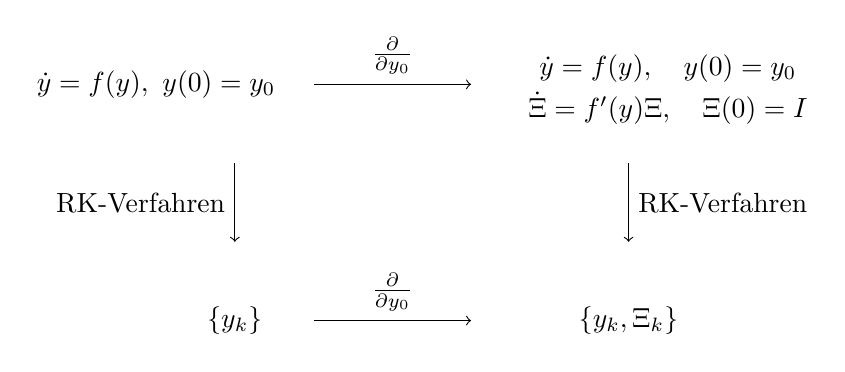
\begin{tikzpicture}
		\draw (0,0)  node{$\{y_k\}$};
		\draw[->] (1,0) -- node[above]{$\frac{\partial}{\partial y_0}$} (3,0); 
		\draw (5,0) node{$\{y_k,\Xi_k\}$};
		\draw[->] (0,2)-- node[left]{RK-Verfahren}(0,1);
		\draw[->] (5,2)-- node[right]{RK-Verfahren}(5,1);
		\draw[->] (1,3)-- node[above]{$\frac{\partial}{\partial y_0}$}(3,3);
		\draw (-1,3)  node{$\dot y = f(y),\ y(0)=y_0$};
		\draw (5.5,3.2)  node{$\dot y = f(y),\quad y(0)=y_0$};
		\draw (5.5,2.7)  node{$\dot\Xi = f'(y)\Xi,\quad \Xi(0)=I$};
		\end{tikzpicture}
	\end{center}
\end{lemma}
\begin{proof}[Beweisidee:] Betrachte exemplarisch das explizite Euler-Verfahren
	\begin{equation*}
		y_{k+1} = y_k +\tau f(y_k).
	\end{equation*}
	Ableiten nach $y_0$ ergibt
	\begin{equation*}
		\Xi_{k+1} = \Xi_k + \tau f'(y_k)\Xi_k.
	\end{equation*}
	Das ist gerade das explizite Euler-Verfahren für die Gleichung
	\begin{equation*}
		\dot \Xi = f'(y)\Xi.
	\end{equation*}
	Startwert passt auch, denn $I=\frac{\partial y_0}{\partial y_0} = \Xi_0$.
\end{proof}


\begin{idea}
	Die Symplektizitätsbedingung ist eine quadratische Invariante des
	erweiterten Systems für die Variablen $y$ und $\Xi$.
\end{idea}

\begin{satz}
	Alle Verfahren die quadratische Invarianten erhalten sind symplektisch.
\end{satz}
\begin{proof}
	Der quadratische Ausdruck $\Xi^T J\Xi$ is Invariante der Gleichung
	\begin{equation*}
		\dot \Xi = J^{-1}\nabla^2 H(y)\Xi,
	\end{equation*}
	denn
	\begin{align*}
		\frac{d}{dt}\Big(\Xi^T J\Xi\Big) & = \dot \Xi^T J\Xi + \Xi^T J\dot\Xi \\
		& = (J^{-1}\nabla^2 H\Xi)^T J\Xi + \Xi^T JJ^{-1}\nabla^2 H \Xi \\
		& = \Xi^T \nabla^2 H \underbrace{J^{-T}J}_{=-I} + \Xi^T\underbrace{ JJ^{-1}}_{=I} \nabla^2 H \Xi \\
		& = 0
	\end{align*}
\end{proof}

\begin{kor}
	Gauß-Verfahren sind symplektisch.
\end{kor}

\subsection{Reversibilität vs.\ Symplektizität}

Es gibt reversible Verfahren, die nicht symplektisch sind.
Es gibt symplektische Verfahren, die nicht reversibel sind.

Für quadratische Hamilton-Funktionen ist das aber anders.

\begin{satz}[{{{\cite[Satz VI.4.9.]{hairer_lubich_wanner:2006}}}}]
	Für RK-Verfahren sind die folgenden Aussagen äquivalent:
	\begin{enumerate}[label=(\roman*)]
		\item Die Methode ist reversibel für lineare Probleme
		\begin{equation*}
			\dot y = Ly
		\end{equation*}
		\item Die Methode ist symplektisch für Hamilton-Gleichungen mit quadratischer Hamilton-Funktion
		\begin{equation*}
			H(y) = \frac{1}{2} y^TCy.\qquad C\ s.p.d.
		\end{equation*}
	\end{enumerate}
\end{satz}
\begin{proof}
	$ii) \to i)$\\
	\begin{itemize}
		\item Die Hamilton-Gleichungen haben die Form
		\begin{equation*}
		\dot y = J^{-1} \nabla H(y) = J^{-1}Cy,
		\end{equation*}
		sind also linear.
		\item Das Runge-Kutta-Verfahren dafür hat also die Form
		\begin{equation*}
		\Psi^\tau y = R(\tau J^{-1} C) y
		\end{equation*}
		wobei $R$ die Stabilitätsfunktion ist.
		\item Da das Verfahren symplektisch ist, gilt
		\begin{equation*}
		R(\tau J^{-1} C)^T J R(\tau J^{-1} C) = J.
		\end{equation*}
		
		\item Da $R= PQ^{-1}$ für Polynome $P,Q$ erhält man
		\begin{equation}\label{eq:beweis_symplektisch_symmetrisch}
		P(\tau J^{-1} C)^T JP(\tau J^{-1} C) = Q(\tau J^{-1} C)^T J Q(\tau J^{-1} C).
		\end{equation}
		
		\item Betrachte das Produkt \glqq Polynom in $J^{-1} C$\grqq\ mit $J$.
		
		\item Für jedes Monom $(J^{-1} C)^k$, $k \in \N$ gilt
		($C$ ist symmetrisch, und $J^T = -J$)
		\begin{align*}
		((J^{-1} C)^k)^T J
		& =
		(C^T J^{-T})^k J \\
		& =
		\underbrace{C^TJ^{-T} \dots C^TJ^{-T}}_{\text{$k$ mal}} J \\
		& =
		-C^T\underbrace{J^{-T}C^T \dots J^{-T}C^T}_{\text{$k-1$ mal}} \\
		& =
		-C\underbrace{J^{-T}C \dots J^{-T}C}_{\text{$k-1$ mal}} \\
		& =
		-J^T J^{-T} C\underbrace{J^{-T}C \dots J^{-T}C}_{\text{$k-1$ mal}} \\
		& =
		-J^T (J^{-T}C)^k \\
		& =
		J(-J^{-1} C)^k.
		\end{align*}
		\item Also folgt aus \eqref{eq:beweis_symplektisch_symmetrisch}
		\begin{equation*}
		P(-\tau J^{-1} C)\cdot P(\tau J^{-1} C) =  Q(-\tau J^{-1} C)\cdot Q(\tau J^{-1} C)
		\end{equation*}
		bzw.
		\begin{equation*}
		R(-\tau J^{-1} C)\cdot R(\tau J^{-1} C) = I.
		\end{equation*}
		\item  Das ist gerade die Reversibilität des Verfahrens.
	\end{itemize}
\end{proof}

\section{Energieerhaltung}

Wir haben einige Mühe in Verständnis und Erhaltung der Symplektizität gesteckt.
Aber Symplektizität ist eine sehr abstrakte Eigenschaft. Wozu soll die gut sein? Hier komme eine etwas konkretere Rechtfertigung.

Betrachte das mathematische Pendel.
\begin{itemize}
	\item Kinetische Energie:
	\begin{equation*}
		T(q, \dot q) = \frac{m l^2}{2} \dot q
	\end{equation*}
	($q$ ist der Winkel)
	\item Potentielle Energie:
	\begin{equation*}
		U(q) = -mgl \cos q
	\end{equation*}
	\item Bewegungsgleichungen:
	\begin{equation*}
		\ddot q + \frac gl \sin q = 0
	\end{equation*}
	\item Gesamtenergie:
	\begin{equation*}
		E = \frac{m l^2}2 \dot q^2 - mgl \cos q
	\end{equation*}
	Dies entspricht der Hamilton-Funktion
	\begin{equation*}
		H(p, q) = \frac{1}{2ml^2} p^2 - mgl \cos q
	\end{equation*}
	Damit ist die Gesamtenergie eine Erhaltungsgröße!
	\item Aber: weder linear noch quadratisch.
	Wird daher nicht automatisch von z.B. Gauß-Verfahren erhalten.
\end{itemize}

Wird die Energie von symplektischen Verfahren erhalten?

Nein! Aber fast...

\begin{satz}[{{{\cite{benettin_giorgilli:1994}; \cite[Thm.\,IX.8.1]{hairer_lubich_wanner:2006}}}}]
	Betrachte ein Hamilton-System mit analytischer Hamilton-Funktion $H: D \to R$ ($D \subset \R^{2d}$) und wende ein symplektisches Verfahren $\Psi^\tau$ mit Schrittweite $\tau$ an. Wenn die numerische Lösung in einer kompakten Menge $K\subset D$ bleibt, dann existiert ein $\tau_0$, so dass
	\begin{equation*}
		H(y_n) = H(y_0) + O(\tau^p) \vadjust{\todo{$H$ ist nicht ganz konstant, aber die Abweichung ist seeeehr klein - nämlich in $\mathcal{O}(\tau^p)$}}
	\end{equation*}
	für exponentiell lange Zeitintervalle $n\tau \le e^{\frac{\tau_0}{2 \tau}}$.
\end{satz}

Symplektische Verfahren erhalten also \emph{nicht} die Hamilton-Funktion bzw.\ die Gesamtenergie. Aber die numerische Energie bleibt \enquote{in der Nähe} der exakten Energie!


\section{Variationelle Integratoren}

Mit dem jetzt Gelernten können wir Zeitschrittverfahren auf eine ganz neue Art konstruieren.
Siehe dazu \cite{marsden_west:2001} für eine detailliertere Übersicht.

Wir erinnern an das Prinzip der stationären Wirkung (auch Hamiltonsches Prinzip genannt): 
Lagrange-Funktion
\begin{equation*}
	L(q,\dot q) = T(q,\dot q) - U(q)
\end{equation*}

\begin{definition}
	Die \begriff{Wirkung} eine Trajektorie $q\colon t\mapsto (q(t),\dot q(t))$ ist
	\begin{equation*}
		S(q)\coloneqq \int_{t_0}^{t_1} L(q(t),\dot q(t))\,dt.
	\end{equation*}
\end{definition}

Wir betrachten nur Trajektorien mit gegebenem festen Start- und Endpunkt
\begin{equation*}
	q(t_0) = q_0,\qquad q(t_1) = q_1.
\end{equation*}

\begin{definition}[Hamiltonsches Prinzip]
	Die tatsächlich vorkommenden Trajektorien sind die, die die Wirkung stationär machen.
\end{definition}

Sei $q$ eine Trajektorie, und $\delta q$ eine Variation davon, die die Endpunkte fest lässt, also $\delta q(t_0)=\delta(t_1) = 0$.
Stationarität von $q$ heißt dann, dass für alle solche $\delta q$
\begin{equation*}
	\frac{d}{d\epsilon} S(q+\epsilon\delta q)\big\vert_{\epsilon=0} = 0.
\end{equation*}
Wie schon in Kapitel~\ref{sec:lagrange_gleichung} gezeigt ist dies äquivalent zur Euler--Lagrange-Gleichung
\begin{equation*}
	\frac{d}{dt}\frac{\partial L}{\partial \dot q} = \frac{\partial L}{\partial q}.
\end{equation*}

Wir betrachten jetzt das Wirkungsintegral $S$ als Funktion der Start- und Endposition
\begin{equation*}
	S(q_0,q_1) = \int_{t_0}^{t_1} L(q(t),\dot q(t))\,dt.
\end{equation*}
Dabei ist $q$ die zu $q_0,q_1$ gehörige Lösung der Lagrange-Gleichung.

\subsubsection*{Exkurs Anfang: Erzeugendenfunktionen}

Wir brauchen ein weiteres Kriterium für Symplektizität:
\begin{itemize}
	\item Betrachte ein gegebenes Hamiltonsches System $H$ auf einem festen Zeitintervall $[t_0,t_1]$
	\item Seien $p_0 \in \R^d$ und $q_0 \in \R^d$ die Startwerte zur Zeit $t_0$
	\item Bezeichne die Werte zur Zeit $t_1$ mit  $p_1 \in \R^d$ und $q_1 \in \R^d$
	\item Es gibt eine Abbildung $\Phi^{t_0,t_1}(p_0,q_0) = (p_1,q_1)$.
\end{itemize}

Wie wir wissen, ist diese symplektisch.
{[Achtung: der folgende Satz enthält überdurchschnittlich viel didaktische Reduktion]}

\begin{satz}[{{\cite[Satz VI.5.1]{hairer_lubich_wanner:2006}}}]
	\label{thm:erzeugendenfunktion}
	Eine Abbildung $\varphi\colon (p_0,q_0) \mapsto (p_1,q_1)$ ist genau dann symplektisch, wenn lokal eine Funktion
	\begin{equation*}
		S\colon (q_0,q_1)\mapsto S(q_0,q_1)\in\R
	\end{equation*}
	existiert, so dass
	\begin{equation}\label{eq:abbildung_symplektisch}
		\nabla S 0
		\begin{pmatrix}
		\frac{\partial S}{\partial q_0}  \\
		\frac{\partial S}{\partial q_1}
		\end{pmatrix} = \begin{pmatrix}
		-p_0 \\ p_1
		\end{pmatrix}
	\end{equation}
\end{satz}

Wenn man eine symplektische Abbildung $(p_0,q_0)\mapsto(p_1,q_1)$ hat, dann kann sie durch \eqref{eq:abbildung_symplektisch} aus der Funktion $S$ rekonstruiert werden.

Aber der obige Satz ist vom Typ \enquote{Äquivalenz}. Es gilt also auch die Umkehrung: Jede hinreichen glatte (und in einem gewissen Sinne nicht degenerierte) Funktion $S$ \emph{erzeugt} via \eqref{eq:abbildung_symplektisch} eine symplektische Abbildung $(p_0,q_0)\mapsto (p_1,q_1)$.\note{Hier muss noch was hin.}

Man kann also auf systematische Art symplektische Abbildungen erzeugen. Die Funktion $S$ heißt deshalb Erzeugendenfunktion.

\subsubsection*{Exkurs Ende}



%%%%%%%%%%%%%%%%%%%%%%%%%%%%%%%%%%%%%%%%%%%%%%%%%%%%%%%%%%%%%%%%%%%%%%%%%%%%%%%%%%%%%%%%%%%%%%%%%%%%%%%%%%%%%%%%%%%%%%%%%%%%%%%%%%%%%%%%%%%%%%%%%%%%


%\section{Symplektizität}
%
%Flüsse von Hamiltonschen Systemen haben eine weitere wichtige Erhaltungseigenschaft,
%\begin{itemize}
%\item die sog. Symplektizität
%\item ähnlich wie Volumenerhaltung im Phasenraum
%\end{itemize}
%
%\emph{Beispiel}: Volumenerhaltung beim mathematischen Pendel
%
%  \bigskip
%  \todoannot{1.5\baselineskip}{Bild}
%
%Betrachte die Hamiltonschen Gleichungen
%\begin{equation*}
%  \dot p = - \frac{\partial H}{\partial q}(p, q),
%  \quad
%  \dot q = \frac{\partial H}{\partial p}(p, q)
%\end{equation*}
%
%Umschreiben:
%\begin{equation*}
%  \begin{pmatrix} \dot p \\ \dot q \end{pmatrix}
%  =
%  \begin{pmatrix} 0 & I \\ -I & 0 \end{pmatrix}^{-1}
%  \begin{pmatrix} \frac{\partial H}{\partial p} \\ \frac{\partial H}{\partial q} \end{pmatrix}
%\end{equation*}
%
%Diese Beziehung wollen wir jetzt abstrakter betrachten.
%
%Bemerke: die harmlos aussehende Matrix $\begin{pmatrix} 0 & I \\ -I & 0 \end{pmatrix}$ hat eine besondere Eigenschaft.
%Es gilt nämlich
%\begin{equation*}
%  \begin{pmatrix} 0 & I \\ -I & 0 \end{pmatrix}^2
%  = - \begin{pmatrix} I & 0 \\ 0 & I \end{pmatrix}.
%\end{equation*}
%\begin{itemize}
%\item Verhält sich also wie die imaginäre Einheit $i$.
%\item Erzeugt eine komplexe Struktur auf $\R^{2d}$.
%\end{itemize}
%
%Wir betrachten 2-dimensionale Parallelogramme in $\R^{2d}$.
%\begin{itemize}
%\item Aufgespannt durch Vektoren
%  \begin{equation*}
%    \xi = \begin{pmatrix} \xi^p \\ \xi^q \end{pmatrix},
%    \quad
%    \eta = \begin{pmatrix} \eta^p \\ \eta^q \end{pmatrix}.
%  \end{equation*}
%\end{itemize}
%
%Falls $d = 1$, so ist die orientierte Fläche des Parallelogramms gerade
%\begin{equation*}
%  \det\begin{pmatrix} \xi^p & \eta^p \\ \xi^q & \eta^q \end{pmatrix}
%  =
%  \xi^p \eta^q - \xi^q \eta^p
%  =
%  (\xi^p \quad \xi^q)
%  \begin{pmatrix} 0 & 1 \\ -1 & 0 \end{pmatrix}
%  \begin{pmatrix} \eta^p \\ \eta^q \end{pmatrix}.
%\end{equation*}
%Das verallgemeinern wir jetzt für höhere Dimensionen.
%
%\begin{definition}[Symplektische Form]
%  Die symplektische Form $\omega: \R^{2d} \times \R^{2d} \to \R$ ist
%  \begin{equation*}
%    \omega(\xi, \eta)
%    \colonequals \sum_{i=1}^d \det\begin{pmatrix} \xi_i^p & \eta_i^p \\ \xi_i^q & \eta_i^q \end{pmatrix}
%    = \sum_{i=1}^d \left( \xi_i^p \eta_i^q - \xi_i^q \eta_i^p \right).
%  \end{equation*}
%\end{definition}
%
%\begin{itemize}
%\item Bilineare Form
%\item Interpretation: Summe der orientierten Flächen der Projektionen auf die Koordinatenebenen $(p_i, q_i)$.
%\item Matrixdarstellung
%  \begin{equation*}
%    \omega(\xi, \eta)
%    =
%    \begin{pmatrix} {\xi^p}^T & {\xi^q}^T \end{pmatrix}
%    \begin{pmatrix} 0 & I \\ -I & 0 \end{pmatrix}
%    \begin{pmatrix} \eta^p \\ \eta^q \end{pmatrix}.
%  \end{equation*}
%\end{itemize}
%
%Da die Matrix $\begin{pmatrix} 0 & I \\ -I & 0 \end{pmatrix}$ wichtig zu sein scheint geben wir ihr den Namen $J$.
%
%Eine wichtige Eigenschaft von Hamiltonschen Systemen ist nun, dass ihre Flüsse
%\begin{equation*}
%  \Phi^t: \R^{2d} \to \R^{2d}
%\end{equation*}
%die symplektische Form erhalten.
%
%Das muss man natürlich erklären.
%
%\begin{definition}[Lineare symplektische Abbildung]
%  Eine lineare Abbildung $A: \R^{2d} \to \R^{2d}$ heißt \emph{symplektisch}, wenn
%  \begin{equation*}
%    \omega(A\xi, A\eta) = \omega(\xi, \eta) \qquad \forall \xi, \eta \in \R^{2d}.
%  \end{equation*}
%  Alternativ: Wenn
%  \begin{equation*}
%    A^T J A = J.
%  \end{equation*}
%\end{definition}
%
%\begin{itemize}
%\item Für $d=1$ bedeutet das gerade, dass $A$ flächenerhaltend ist.
%\end{itemize}
%
%\begin{definition}[Differenzierbare symplektische Abbildung]
%  Sei $U$ eine offene Teilmenge von $\R^{2d}$.
%  Eine differenzierbare Abbildung $g: U \to \R^{2d}$ heißt \emph{symplektisch}, falls die Jacobi-Matrix $\nabla g(p,q)$ für alle $(p, q) \in U$ symplektisch ist.
%\end{definition}
%
%Jetzt der zentrale Satz:
%die Flüsse $\Phi^t$ von Hamiltonschen Systemen erhalten die symplektische Form:
%
%\begin{satz}[Poincaré, 1899]
%  Sei $H(p, q)$ zweimal stetig differenzierbar auf $U \subset \R^{2d}$.
%  Sei $\Phi^t$ der Phasenfluss der Differentialgleichung
%  \begin{equation*}
%    \dot y = J^{-1} \nabla H(y)
%  \end{equation*}
%  mit $y = (p, q)$.
%
%  Für jedes feste $t$ ist $\Phi^t$ eine symplektische Abbildung.
%\end{satz}
%
%\begin{proof}
% Der Beweis erfolgt in zwei Schritten:
%  \begin{enumerate}
%  \item $\Phi^0$ ist symplektisch.
%  \item Die \glqq Abweichung von der Symplektizität\grqq{} hängt nicht von $t$ ab.
%  \end{enumerate}
%
%  Zu 1):
%  \begin{itemize}
%  \item $\Phi^0$ ist symplektisch, wenn seine erste Ableitung an jedem Punkt $y_0 = (p_0, q_0)$ symplektisch ist.
%  \item Da $\Phi^0 y_0 = y_0$ gilt
%    \begin{equation*}
%      \left( \frac{\partial \Phi^0 y_0}{\partial y_0} \right)^T J \left( \frac{\partial \Phi^0 y_0}{\partial y_0} \right)
%      = I^T J I
%      = J.
%    \end{equation*}
%  \item Also ist $\Phi^0$ symplektisch.
%  \end{itemize}
%
%  Zu 2):
%  \begin{itemize}
%  \item Wir müssen die Ableitung $\frac{\partial \Phi^t y_0}{\partial y_0}$ untersuchen.
%  \item Linearisierte Störung der Lösung bei einer Störung des Startwerts.
%  \item Also gerade die Wronski-Matrix $\Xi$
%  \item Löst die Gleichung
%    \begin{equation*}
%      \dot \Xi = J^{-1} \underbrace{\nabla^2 H( \Phi^t(y_0) )}_{\text{Hesse-Matrix von $H$}} \Xi
%    \end{equation*}
%
%  \item Konkret heißt das hier
%    \begin{equation}
%     \label{eq:wronski_symplectic_form}
%      \frac{d}{dt} \frac{\partial \Phi^t}{\partial y_0}
%      = J^{-1} \nabla^2 H(\Phi^t y_0) \frac{\partial \Phi^t}{\partial y_0}
%    \end{equation}
%
%
%  \item Produktregel:
%   \begin{equation*}
%    \frac{d}{dt}\bigg[ \bigg(\frac{\partial \Phi^t}{\partial y_0}\bigg)^T J \bigg(\frac{\partial \Phi^t}{\partial y_0}\bigg) \bigg]
%    = \bigg( \frac{d}{dt} \frac{\partial \Phi^t}{\partial y_0} \bigg)^T J \bigg( \frac{\partial \Phi^t}{\partial y_0} \bigg)
%    + \bigg( \frac{\partial \Phi^t}{\partial y_0} \bigg)^T J \bigg( \frac{d}{dt} \frac{\partial \Phi^t}{\partial y_0} \bigg)
%    \end{equation*}
%
%   \item Dort wird jetzt \eqref{eq:wronski_symplectic_form} eingesetzt:
%    \begin{equation*}
%      \frac{d}{dt}\bigg[ \bigg(\frac{\partial \Phi^t}{\partial y_0}\bigg)^T J \bigg(\frac{\partial \Phi^t}{\partial y_0}\bigg) \bigg]
%      =
%      \bigg(\frac{\partial \Phi^t}{\partial y_0}\bigg)^T \nabla^2 H(\Phi^t y_0)^T J^{-T} J \bigg(\frac{\partial \Phi^t}{\partial y_0}\bigg)
%      + \bigg(\frac{\partial \Phi^t}{\partial y_0}\bigg)^T J J^{-1} \nabla^2 H(\Phi^t y_0) \bigg(\frac{\partial \Phi^t}{\partial y_0}\bigg)
%    \end{equation*}
%  \item Aber $J^T = -J$, also $J^{-T} J = -I$, und $\nabla^ H$ ist symmetrisch.
%  \item Deshalb ist
%    \begin{equation*}
%      \frac{d}{dt}\bigg[ \bigg(\frac{\partial \Phi^t}{\partial y_0}\bigg)^T
%        J
%        \bigg(\frac{\partial \Phi^t}{\partial y_0}\bigg) \bigg]
%      = 0.
%      \qedhere
%    \end{equation*}
%  \end{itemize}
%\end{proof}
%
%Es gilt sogar die Umkehrung des Satzes:
%\emph{nur} Hamiltonsche Systeme haben symplektische Flüsse!
%
%\begin{definition}[lokal Hamiltonsch]
%  Eine Differentialgleichung $x' = f(x)$ heißt \emph{lokal Hamiltonsch}, wenn für jedes $x_0 \in U$ eine Nachbarschaft existiert, in der
%  \begin{equation*}
%    f(x) = J^{-1} \nabla H(x)
%  \end{equation*}
%  für eine Funktion $H$.
%\end{definition}
%
%\begin{satz}[{\citet[Satz~VI.2.6]{hairer_lubich_wanner:2006}}]
%  Sei $f: U \to \R^{2d}$ stetig differenzierbar.
%  Dann ist $x' = f(x)$ genau dann lokal Hamiltonsch, wenn der Fluss $\Phi^t x$ für alle $x \in U$ und alle $t$ hinreichend klein symplektisch ist.
%\end{satz}
%
%\section{Symplektische Verfahren}
%
%Wir wollen Verfahren entwickeln, die die Symplektizität von Hamiltonschen Flüssen erben.
%
%\begin{definition}
%	Ein Einschrittverfahren heißt symplektisch, falls der diskrete Fluss
%	\begin{equation*}
%		\Psi^t\colon \R^{2d}\to\R^{2d}
%	\end{equation*}
%	symplektisch ist, wenn das Verfahren auf ein Hamiltonsches System angewendet wird.
%\end{definition}
%
%Die einfachsten symplektischen Verfahren sind die symplektischen Euler-Verfahren
%\begin{align*}
%	p_{k+1} &= p_k - \tau H_q(p_{k+1},q_k) \\
%	q_{k+1} &= q_k + \tau H_p(p_{k+1},q_k)
%\end{align*}
%und
%\begin{align*}
%	p_{k+1} &= p_k - \tau H_q(p_k,q_{k+1}) \\
%	q_{k+1} &= q_k + \tau H_p(p_k,q_{k+1}).
%\end{align*}
%
%\begin{satz}[{\citet[Satz~VI.3.3]{hairer_lubich_wanner:2006}}]
%	Die symplektischen Euler-Verfahren sind symplektisch.
%\end{satz}
%\begin{proof}
%	Beweis für die erste Methode:
%	\begin{itemize}
%		\item Methode ist symplektisch, wenn
%		\begin{equation*}
%			\frac{\partial\Psi^\tau y}{\partial y}\in \R^{2d\times 2d}
%		\end{equation*}
%		für alle $y=(p,q)$ die symplektisch Form erhält, wenn also
%		\begin{equation}\label{eq:symplektische_form}
%			\Big(\frac{\partial\Psi^\tau y}{\partial y}\Big)^TJ\Big(\frac{\partial\Psi^\tau y}{\partial y}\Big) = J.
%		\end{equation}
%		\item Wir bestimmen die vier Komponenten von $\frac{\partial\Psi^\tau y}{\partial y}$:
%		\item [1)] Erste Gleichung des Verfahrens:
%			\begin{equation*}
%				p_{k+1} = p_k - \tau H_q(p_{k+1},q_k)
%			\end{equation*}
%			Ableiten nach $p_k$:
%			\begin{equation*}
%				\frac{\partial p_{k+1}}{\partial p_k} = I - \tau H_{qp}(p_{k+1},q_k)\cdot \frac{\partial p_{k+1}}{\partial p_k}
%			\end{equation*}
%			$\Leftrightarrow$
%			\begin{equation*}
%				\frac{\partial p_{k+1}}{\partial p_k}\Big(I + \tau H_{qp}\Big) = I
%			\end{equation*}
%			Ebenso z.B.
%			\begin{equation*}
%				\frac{\partial p_{k+1}}{\partial q_k}\Big(I + \tau H_{qp}\Big) = -\tau H_{qq}
%			\end{equation*}
%			etc.
%	\end{itemize}
%Zusammen erhält man
%\begin{equation*}
%	\begin{pmatrix}
%		I + \tau H_{qp}^T & 0 \\ -\tau H_{pp} & I
%	\end{pmatrix}
%	\begin{pmatrix}
%		\frac{\partial p_{k+1}}{\partial p_k} & 	\frac{\partial p_{k+1}}{\partial q_k} \\
%			\frac{\partial q_{k+1}}{\partial p_k}  & 	\frac{\partial q_{k+1}}{\partial q_k}
%	\end{pmatrix}
%	=
%	\begin{pmatrix}
%		I & -\tau H_{qq} \\ 0 & I+\tau H_{qp}
%	\end{pmatrix},
%\end{equation*}
%also
%\begin{equation*}
%	\frac{\partial \Psi^\tau y}{\partial y} = \begin{pmatrix}
%	I + \tau H_{qp}^T & 0 \\ -\tau H_{pp} & I
%	\end{pmatrix}^{-1} \begin{pmatrix}
%	I & -\tau H_{qq} \\ 0 & I+\tau H_{qp}
%	\end{pmatrix}.
%\end{equation*}
%Damit kann man die Erhaltungseigenschaft \eqref{eq:symplektische_form} direkt nachrechnen.
%\end{proof}
%
%\medskip
%
%Die symplektischen Euler-Verfahren sind \emph{keine} RK-Verfahren.\\
%Stattdessen gehören sie zu den sog.\ \emph{partitionierten} RK-Verfahren.\\
%Betrachte Differentialgleichungen der Form
%\begin{equation*}
%	y'=f(y,z),\qquad z'=g(y,z),
%\end{equation*}
%wobei $y\in\R^{n_1}$ und $z\in\R^{n_2}$\\
%\emph{Idee:} Nimm für $y$ und $z$ zwei verschiedene RK-Verfahren.\\
%Details bei \citet[Kapitel II.2]{hairer_lubich_wanner:2006}
%
%\medskip
%
%Es gibt auch ein \glqq einfaches\grqq\ Verfahren zweiter Ordnung, das symplektisch ist.
%\begin{satz}[{\citet[Satz~VI.3.5]{hairer_lubich_wanner:2006}}]
%	Die implizite Mittelpunktsregel
%	\begin{equation*}
%		y_{k+1} = y_k + \tau J^{-1}\nabla H\Big( \frac{y_{k+1}+y_k}{2}\Big)
%	\end{equation*}
%	ist symplektisch.
%\end{satz}
%\begin{proof}
%	Wir leiten wieder ab
%	\begin{align*}
%		\frac{\partial \Psi^\tau y_k}{\partial y_k} &= \frac{\partial y_{k+1}}{\partial y_k} \\
%		&= I + \tau J^{-1} \nabla^2 H\Big( \frac{y_{k+1} + y_k}{2} \Big) \cdot \Big( \frac{1}{2} \frac{\partial y_{k+1}}{y_k} + \frac{1}{2}\Big).
%	\end{align*}
%Umformen ergibt
%\begin{align*}
% \frac{\partial y_{k+1}}{\partial y_k}
% &=
% \Big( I - \frac{\tau}{2} J^{-1}\nabla^2H\Big)^{-1}\Big(I+\frac{\tau}{2}J^{-1}\nabla^2 H\Big).
%\end{align*}
%
%	Dann kann man direkt nachrechnen dass
%	$\Big(\frac{\partial y_{k+1}}{\partial y_k}\Big)^T J \frac{\partial y_{k+1}}{\partial y_k} = J$.
%
% \bigskip
%\todoannot{1.5\baselineskip}{Ein paar Details zu dieser Rechnung einfügen!}
%\end{proof}
%
%
%\subsection{Symplektische RK-Verfahren}
%
%\begin{itemize}
%	\item Relativ neue Verfahren, wurden erst Ende der 1980er Jahre systematisch untersucht.
%\end{itemize}
%
%Wir interessieren uns wieder für die Ableitung
%\begin{equation*}
%\Xi(t) = \frac{\partial \Phi^t y_0}{\partial y_0}.
%\end{equation*}
%Diese löst bekanntlich eine lineare Differentialgleichung.
%
%\begin{lemma}[{\citet[Lemma VI.4.1]{hairer_lubich_wanner:2006}}]
%	
%	Das folgende Diagramm kommutiert für alle Runge-Kutta-Verfahren und alle partitionierten Runge-Kutta-Verfahren:\\
%	\begin{center}
%	    \begin{tikzpicture}
%	    	\draw (0,0)  node{$\{y_k\}$};
%	    	\draw[->] (1,0) -- node[above]{$\frac{\partial}{\partial y_0}$} (3,0); 
%	    	\draw (5,0) node{$\{y_k,\Xi_k\}$};
%	    	\draw[->] (0,2)-- node[left]{RK-Verfahren}(0,1);
%	    	\draw[->] (5,2)-- node[right]{RK-Verfahren}(5,1);
%	    	\draw[->] (1,3)-- node[above]{$\frac{\partial}{\partial y_0}$}(3,3);
%	    	\draw (-1,3)  node{$\dot y = f(y),\ y(0)=y_0$};
%	    	\draw (5.5,3.2)  node{$\dot y = f(y),\quad y(0)=y_0$};
%	    	\draw (5.5,2.7)  node{$\dot\Xi = f'(y)\Xi,\quad \Xi(0)=I$};
%	    \end{tikzpicture}
%	\end{center}
%\end{lemma}
%\begin{proof}[Beweisidee:] Betrachte exemplarisch das explizite Euler-Verfahren
%\begin{equation*}
%	y_{k+1} = y_k +\tau f(y_k).
%\end{equation*}
%Ableiten nach $y_0$ ergibt
%\begin{equation*}
%	\Xi_{k+1} = \Xi_k + \tau f'(y_k)\Xi_k.
%\end{equation*}
%Das ist gerade das explizite Euler-Verfahren für die Gleichung
%\begin{equation*}
%	\dot \Xi = f'(y)\Xi.
%\end{equation*}
%Startwert passt auch, denn $I=\frac{\partial y_0}{\partial y_0} = \Xi_0$.
%\end{proof}
%
%\bigskip
%
%\emph{Idee:} Die Symplektizitätsbedingung ist eine quadratische invariante des
%erweiterten Systems für die Variablen $y$, $\Xi$.
%
%
%\begin{satz}
%	Alle Verfahren die quadratische Invarianten erhalten sind symplektisch.
%\end{satz}
%\begin{proof}
%	Der quadratische Ausdruck $\Xi^T J\Xi$ is Invariante der Gleichung
%	\begin{equation*}
%		\dot \Xi = J^{-1}\nabla^2 H(y)\Xi,
%	\end{equation*}
%	denn
%	\begin{align*}
%		\frac{d}{dt}\Big(\Xi^T J\Xi\Big) & = \dot \Xi^T J\Xi + \Xi^T J\dot\Xi \\
%		                                 & = (J^{-1}\nabla^2 H\Xi)^T J\Xi + \Xi^T JJ^{-1}\nabla^2 H \Xi \\
%		                                 & = \Xi^T \nabla^2 H \underbrace{J^{-T}J}_{=-I} + \Xi^T\underbrace{ JJ^{-1}}_{=I} \nabla^2 H \Xi \\
%		                                 & = 0.  \qedhere
%	\end{align*}
%\end{proof}
%
%\begin{kor}
%	Gauß-Verfahren sind symplektisch.
%\end{kor}
%
%\subsection{Reversibilität vs.\ Symplektizität}
%
%Es gibt reversible Verfahren, die nicht symplektisch sind.
%
%\medskip
%
%Es gibt symplektische Verfahren, die nicht reversibel sind.
%
%\medskip
%
%Für quadratische Hamilton-Funktionen ist das anders.
%
%\begin{satz}[{\citet[Satz VI.4.9.]{hairer_lubich_wanner:2006}}]
%	Für RK-Verfahren sind die folgenden Aussagen äquivalent:
%	\begin{itemize}
%		\item [i)] Die Methode ist reversibel für lineare Probleme
%		\begin{equation*}
%			\dot y = Ly
%		\end{equation*}
%		\item [ii)] Die Methode ist symplektisch für Hamilton-Gleichungen mit quadratischer Hamilton-Funktion
%		\begin{equation*}
%			H(y) = \frac{1}{2} y^TCy.\qquad C\ s.p.d.
%		\end{equation*}
%	\end{itemize}
%\end{satz}
%\begin{proof}
%	$ii) \to i)$\\
%	\begin{itemize}
%		\item Die Hamilton-Gleichungen haben die Form
%		\begin{equation*}
%			\dot y = J^{-1} \nabla H(y) = J^{-1}Cy,
%		\end{equation*}
%		sind also linear.
%
%		\item Das Runge-Kutta-Verfahren dafür hat also die Form
%		\begin{equation*}
%			\Psi^\tau y = R(\tau J^{-1} C) y
%		\end{equation*}
%		wobei $R$ die Stabilitätsfunktion ist.
%		\item Da das Verfahren symplektisch ist, gilt
%		\begin{equation*}
%			R(\tau J^{-1} C)^T J R(\tau J^{-1} C) = J.
%		\end{equation*}
%
%		\item Da $R= PQ^{-1}$ für Polynome $P,Q$ erhält man
%		\begin{equation}\label{eq:beweis_symplektisch_symmetrisch}
%			P(\tau J^{-1} C)^T JP(\tau J^{-1} C) = Q(\tau J^{-1} C)^T J Q(\tau J^{-1} C).
%		\end{equation}
%
%\todoannot{1.5\baselineskip}{Die folgende Rechnung muss nochmal im Detail überprüft werden!}
%
%		\item Betrachte das Produkt \glqq Polynom in $J^{-1} C$\grqq\ mit $J$.
%
%		\item Für jedes Monom $(J^{-1} C)^k$ gilt ($C$ ist symmetrisch)
%		\begin{equation*}
%			((J^{-1} C)^k)^T J
%			=
%			(C^T J^{-T})^k J
%			=
%			J(-(J^{-1} C)^k)\quad \forall k=0,1,2,\hdots
%		\end{equation*}
%		\item Also folgt aus \eqref{eq:beweis_symplektisch_symmetrisch}
%		\begin{equation*}
%			P(-\tau J^{-1} C)\cdot P(\tau J^{-1} C) =  Q(-\tau J^{-1} C)\cdot Q(\tau J^{-1} C)
%		\end{equation*}
%		bzw.
%		\begin{equation*}
%			R(-\tau J^{-1} C)\cdot R(\tau J^{-1} C) = I.
%		\end{equation*}
%		\item  Das ist gerade die Symmetrie des Verfahrens.
%		\qedhere
%	\end{itemize}
%\end{proof}
%
%\section{Energieerhaltung}
%
%\begin{itemize}
%\item Wir haben einige Mühe in Verständnis und Erhaltung der Symplektizität gesteckt.
%\item Aber Symplektizität ist eine sehr abstrakte Eigenschaft.
%  Wozu soll die gut sein?
%\item Hier komme eine etwas konkretere Rechtfertigung.
%\end{itemize}
%
%Betrachte das mathematische Pendel.
%\begin{itemize}
%\item Kinetische Energie:
%  \begin{equation*}
%    T(q, \dot q) = \frac{m l^2}{2} \dot q
%  \end{equation*}
%  ($q$ ist der Winkel)
%\item Potentielle Energie:
%  \begin{equation*}
%    U(q) = -mgl \cos q
%  \end{equation*}
%\item Bewegungsgleichungen:
%  \begin{equation*}
%    \ddot q + \frac gl \sin q = 0
%  \end{equation*}
%\item Gesamtenergie:
%  \begin{equation*}
%    E = \frac{m l^2}2 \dot q^2 - mgl \cos q
%  \end{equation*}
%  Dies entspricht der Hamilton-Funktion
%  \begin{equation*}
%    H(p, q) = \frac{1}{2ml^2} p^2 - mgl \cos q
%  \end{equation*}
%  Damit ist die Gesamtenergie eine Erhaltungsgröße!
%\item Aber: weder linear noch quadratisch.
%  Wird daher nicht automatisch von z.B. Gauß-Verfahren erhalten.
%\end{itemize}
%
%Wird die Energie von symplektischen Verfahren erhalten?
%
%Nein! Aber fast...
%
%\begin{satz}[{\citet{benettin_giorgilli:1994}; \citet[Thm.\,IX.8.1]{hairer_lubich_wanner:2006}}]
%  Betrachte ein Hamilton-System mit analytischer Hamilton-Funktion $H: D \to R$, ($D \subset \R^{2d}$),
%  und wende ein symplektisches Verfahren $\Psi^\tau$ mit Schrittweite $\tau$ an.
%  Wenn die numerische Lösung in einer kompakten Menge $K\subset D$ bleibt, dann existiert ein $\tau_0$, so dass
%  \begin{equation*}
%    H(y_n) = H(y_0) + O(\tau^p)
%  \end{equation*}
%  für exponentiell lange Zeitintervalle $n\tau \le e^{\frac{\tau_0}{2 \tau}}$.
%\end{satz}
%
%Symplektische Verfahren erhalten also \emph{nicht} die Hamilton-Funktion bzw.\ die Gesamtenergie.
%Aber die numerische Energie bleibt \glqq in der Nähe\grqq{} der exakten Energie!
%
%
%
%\section{Variationelle Integratoren}
%
%Mit dem jetzt Gelernten können wir Zeitschrittverfahren auf eine ganz neue Art konstruieren.\\
%Siehe \citet{marsden_west:2001} für eine detailliertere Übersicht.\\
%
%Wir erinnern an das Prinzip der stationären Wirkung (auch Hamiltonsches Prinzip genannt)
%\begin{itemize}
%	\item Lagrange-Funktion
%	\begin{equation*}
%		L(q,\dot q) = T(q,\dot q) - U(q)
%	\end{equation*}
%\end{itemize}
%
%\begin{definition}
% Die \emph{Wirkung} eine Trajektorie $q\colon t\mapsto (q(t),\dot q(t))$ ist
%	\begin{equation*}
%		S(q)\coloneqq \int_{t_0}^{t_1} L(q(t),\dot q(t))\,dt.
%	\end{equation*}
%\end{definition}
%
%\medskip
%
% Wir betrachten nur Trajektorien mit gegebenem festen Start- und Endpunkt
%	\begin{equation*}
%		q(t_0) = q_0,\qquad q(t_1) = q_1.
%	\end{equation*}
%
%\begin{definition}[Hamiltonsches Prinzip]
%Die tatsächlich vorkommenden Trajektorien sind die, die die Wirkung stationär machen.
%\end{definition}
%
%Sei $q$ eine Trajektorie, und $\delta q$ eine Variation davon, die die Endpunkte fest lässt, also $\delta q(t_0)=\delta(t_1) = 0$.
%\begin{itemize}
%	\item Stationarität von $q$ heißt dann, dass für alle solche $\delta q$
%	\begin{equation*}
%		\frac{d}{d\epsilon} S(q+\epsilon\delta q)\Big\vert_{\epsilon=0} = 0.
%	\end{equation*}
%\end{itemize}
%Wie schon in Kapitel~\ref{sec:lagrange_gleichung} gezeigt ist dies äquivalent zur Euler--Lagrange-Gleichung
%\begin{equation*}
%	\frac{d}{dt}\frac{\partial L}{\partial \dot q} = \frac{\partial L}{\partial q}.
%\end{equation*}
%
%\bigskip
%
%Wir betrachten jetzt das Wirkungsintegral $S$ als Funktion der Start- und Endposition
%\begin{equation*}
%	S(q_0,q_1) = \int_{t_0}^{t_1} L(q(t),\dot q(t))\,dt.
%\end{equation*}
%Dabei ist $q$ die zu $q_0,q_1$ gehörige Lösung der Lagrange-Gleichung.\\
%
%\subsubsection*{Exkurs Anfang: Erzeugendenfunktionen}
%
%Wir brauchen ein weiteres Kriterium für Symplektizität:
%\begin{itemize}
%	\item Betrachte ein gegebenes Hamiltonsches System $H$ auf einem festen Zeitintervall $[t_0,t_1]$
%	\item Seien $p_0 \in \R^d$ und $q_0 \in \R^d$ die Startwerte zur Zeit $t_0$
%	\item Bezeichne die Werte zur Zeit $t_1$ mit  $p_1 \in \R^d$ und $q_1 \in \R^d$
%	\item Es gibt eine Abbildung $\Phi^{t_0,t_1}(p_0,q_0) = (p_1,q_1)$.
%\end{itemize}
%
%Wie wir wissen, ist diese symplektisch.\\
%{[Achtung: der folgende Satz enthält überdurchschnittlich viel didaktische Reduktion]}
%
%\begin{satz}[{\citet[Satz VI.5.1]{hairer_lubich_wanner:2006}}]
%\label{thm:erzeugendenfunktion}
%	Eine Abbildung $\varphi\colon (p_0,q_0) \mapsto (p_1,q_1)$ ist genau dann symplektisch, wenn lokal eine Funktion
%	\begin{equation*}
%	S\colon (q_0,q_1)\mapsto S(q_0,q_1)\in\R
%	\end{equation*}
%	existiert, so dass
%	\begin{equation}\label{eq:abbildung_symplektisch}
%	\nabla S
%	=
%	\begin{pmatrix}
%		\frac{\partial S}{\partial q_0}  \\
%		\frac{\partial S}{\partial q_1}
%	\end{pmatrix} = \begin{pmatrix}
%		-p_0 \\ p_1
%	\end{pmatrix}.
%	\end{equation}
%\end{satz}
%
%\begin{itemize}
%	\item Wenn man eine symplektische Abbildung $(p_0,q_0)\mapsto(p_1,q_1)$ hat, dann sie durch \eqref{eq:abbildung_symplektisch} aus der Funktion $S$ rekonstruiert werden.
%	\item Aber der obige Satz ist \glqq genau dann, wenn\grqq\ . Es gilt also auch die Umkehrung:
%	\begin{itemize}
%		\item Jede hinreichen glatte (und in einem gewissen Sinne nicht degenerierte)
%		 Funktion $S$ \emph{erzeugt} via \eqref{eq:abbildung_symplektisch} eine symplektische Abbildung $(p_0,q_0)\mapsto (p_1,q_1)$!
%	\end{itemize}
%	\item Man kann also auf systematische Art symplektische Abbildungen erzeugen. Die Funktion $S$ heißt deshalb Erzeugendenfunktion.
%\end{itemize}
%
%
%\subsubsection*{Exkurs Ende}
%
%Große Überraschung: Diese Funktion $S$ ist gerade die Erzeugendenfunktion einer symplektischen Abbildung!
%\begin{itemize}
% \item Berechne partielle Ableitung:
%  \begin{align*}
%   \frac{\partial S}{\partial q_0}
%   & =
%   \int_{t_0}^{t_1} \bigg( \frac{\partial L}{\partial q} \frac{\partial q}{\partial q_0} + \frac{\partial L}{\partial \dot q}\frac{\partial\dot q}{\partial q_0}\bigg)\,dt \\
%   %
%   \intertext{Partielle Integration des zweiten Terms in der Klammer liefert}
%   &=
%   \frac{\partial L}{\partial \dot q}\frac{\partial q}{\partial q_0}\Bigg\vert_{t_0}^{t_1} + \int_{t_0}^{t_1} \underbrace{\bigg( \frac{\partial L}{\partial q}  - \frac{d}{dt} \frac{\partial L}{\partial \dot q}\bigg)}_{=0} \frac{\partial q}{\partial q_0}\,dt \\
%		&= \frac{\partial L(q_1,\dot q_1)}{\partial \dot q} \cdot \underbrace{\frac{\partial q_1}{\partial q_0}}_{=0}  - \frac{\partial L(q_0,\dot q_0)}{\partial \dot q} \cdot \underbrace{\frac{\partial q_0}{\partial q_0}}_{=1}  \\
%		&= - \frac{\partial L(q_0,\dot q_0)}{\partial \dot q} \\
%		&= -p_0 \qquad\text{(Def. des Impulses)}.
%	\end{align*}
%\end{itemize}
%Ebenso berechnet man
%\begin{equation*}
%	\frac{\partial S}{\partial q_1} = p_1.
%\end{equation*}
%Wir erhalten also
%\begin{equation}
%\nabla S =
%\begin{pmatrix}
%\frac{\partial S}{\partial q_0}  \\
%\frac{\partial S}{\partial q_1}
%\end{pmatrix}
%=
%\begin{pmatrix}
%-p_0 \\ p_1
%\end{pmatrix}.
%\end{equation}
%Dies ist gerade die Formel \eqref{eq:abbildung_symplektisch} für Erzeugendenfunktionen von symplektischen Abbildungen.
%
%Daraus folgt dass die entsprechende Abbildung $(p_0,q_0) \mapsto (p_1,q_1)$ symplektisch ist.
%
%\subsection{Idee der variationellen Integratoren}
%
%Wir ersetzen das Integral im Hamiltonschen Prinzip durch eine diskrete Approximation:
%
%\medskip
%
%\begin{itemize}
%	\item Führe ein Zeitgitter ein
%	\begin{equation*}
%	t_0<t_1<\hdots < t_N = T.
%	\end{equation*}
%	\item  Führe die approximative Wirkung ein
%	\begin{equation*}
%		L_h(q_k,q_{k+1})\approx \int_{t_k}^{t_{k+1}} L(q(t),\dot q(t))\,dt
%	\end{equation*}
%	(z.B.\ durch eine Quadraturformel)\\
%
%	Hier könnte man denken dass $L_h$ ein schlechtes Symbol ist, weil es sich ja schließlich
%	um eine Wirkung handelt.  Andererseits fungiert $L_h$ später bei der Definition der
%	diskreten Impulse wie eine Lagrange-Funktion (siehe~\eqref{eq:diskrete_lagrange_transformation}).
%
%	$q$ ist hier die Lösung der Lagrange-Gleichung auf $[t_k,t_{k+1}]$ mit gegebenen Start- und Endwerten $q_k,q_{k+1}$.
%	\item Definiere das diskrete Wirkungsfunktional
%	\begin{equation*}
%		S_h\Big(\big\{q_k\big\}_{k=0}^N\Big) \colonequals \sum_{k=0}^{N-1} L_h(q_k,q_{k+1}).
%	\end{equation*}
%\end{itemize}
%
%\begin{definition}[Diskretes Hamilton-Prinzip]
%Finde $\{q_k\}^N_{k=0}$  mit gegebenen $q_0, q_N$, so dass $S_h$ stationär wird.
%\end{definition}
%
%\medskip
%
%Wie kann man $L_h$ wählen?
%
%\medskip
%
%\emph{Beispiel:} (\citet{mackay:1992}, 1992)
%\begin{itemize}
%\item Approximiere $q$ auf $[t_k, t_{k+1}]$ als linear Interpolierende von $q_k$ und $q_{k+1}$.
%\item Approximiere das Integral durch die Trapezregel
%\begin{equation*}
%L_h(q_k, q_{k+1})
%=
%\tau \cdot \frac{1}{2} \Big[L\Big(q_k, \frac{q_{k+1} - q_k}{\tau}\Big) +  L\Big(q_{k+1}, \frac{q_{k+1} - q_k}{\tau}\Big)\Big].
%\end{equation*}
%\end{itemize}
%
%Beispiel: (\citet{wendlandt_marsden:1997}, 1997)
%\begin{itemize}
%\item Nimm statt der Trapezregel die Mittelpunktsregel
%\begin{equation*}
%L_h(q_k, q_{k+1}) = \tau \Big[L\Big(\frac{q_{k+1} + q_k}{2}, \frac{q_{k+1} - q_k}{\tau}\Big)\Big].
%\end{equation*}
%\end{itemize}
%
%Wie kommen wir an stationäre Punkte von $S_h$?
%\begin{itemize}
%\item Ableitung ausrechnen und gleich Null setzen!
%\newline Partielle Ableitung für $k=1, \dots, N-1$:
%\begin{equation*}
%\frac{\partial S_h}{\partial q_k}
%=
%\frac{\partial}{\partial q_k} \sum_{i=0}^{N-1} L_h (q_i, q_{i+1})
%=
%\frac{\partial}{\partial q_k} L_h(q_{k-1}, q_k) +  \frac{\partial}{\partial q_k} L_h(q_k, q_{k+1}).
%\end{equation*}
%\item Dieser Ausdruck $=0$ sind die \emph{diskreten Euler--Lagrange-Gleichungen}.
%\item Ein System von algebraischen Gleichungen (mit Bandstruktur).
%\end{itemize}
%
%\medskip
%
%\textbf{Fragen:}
%\begin{itemize}
%\item Wann kriege ich mit diesem Ansatz symplektische Integratoren?
%\item Kann ich das Verfahren so umschreiben dass ich wieder einen Zeitschritt nach dem anderen berechnen kann?
%\end{itemize}
%
%\subsection{Variationelle Integratoren sind symplektisch}
%
%Wir schreiben die diskrete Wirkung jetzt wieder als Funktion von Anfangs- und Endzustand
%\begin{equation*}
%S_h(q_0, q_N) = \sum_{k=0}^{N-1} L_h (q_k, q_{k+1}).
%\end{equation*}
%Dabei ist $\{q_k\}$ die dazugehörige Lösung des variationellen Integrators.
%\begin{itemize}
%\item Wir rechnen wieder die partiellen Ableitungen aus. Es bezeichne $\frac{\partial L_h}{\partial x}$,
%   $\frac{\partial L_h}{\partial y}$ die partiellen Ableitungen von $L_h$ nach dem ersten bzw.\ zweiten Argument:
%\begin{align*}
%\frac{\partial S_h}{\partial q_0}
%& = \sum_{k=0}^{N-1} \Bigg[ \frac{\partial L_h}{\partial x} \cdot\frac{\partial q_k}{\partial q_0} +  \frac{\partial L_h}{\partial y} \cdot\frac{\partial q_{k+1}}{\partial q_0}\Bigg] \\
%%
%& = \frac{\partial L}{\partial x} (q_0,q_1)\cdot \underbrace{\frac{\partial q_0}{\partial q_0}}_{=1} \\
%& \qquad  + \sum_{k=1}^{N-1} \Bigg[ \underbrace{\frac{\partial L_h}{\partial y}(q_{k-1},q_k) \cdot\frac{\partial q_k}{\partial q_0} +  \frac{\partial L_h}{\partial x} (q_k,q_{k+1})\cdot\frac{\partial q_k}{\partial q_0}}_{\text{$=0$, wg.\ diskreter Lagrange-Gleichung}}\Bigg] \\
%& \qquad \qquad  + \frac{\partial L_h}{\partial y} (q_{N-1},q_N)\cdot \underbrace{\frac{\partial q_N}{\partial q_0}}_{=0} \\
%%
%& =
%\frac{\partial L}{\partial x} (q_0, q_1).
%\end{align*}
%\item Ebenso 
%\begin{equation*}
%\frac{\partial S_h}{\partial q_N}  = \frac{\partial L_h}{\partial y} (q_{N-1}, q_N).
%\end{equation*}
%\end{itemize}
%Jetzt führen wir die \emph{diskreten Impulse} durch eine \emph{diskrete Legendre-Transformation} ein:
%\begin{equation}
%\label{eq:diskrete_lagrange_transformation}
% p_k
% \colonequals
% - \frac{\partial L_h}{\partial x} (q_k, q_{k+1})
% =
% \frac{\partial L_h}{\partial y} (q_{k-1}, q_k)
%\end{equation}
%Die Gleichheit ist gerade die diskrete Euler--Lagrange-Gleichung.
%
%[Vergleiche: $p = \frac{\partial L}{\partial \dot{q}}(q,\dot{q})$]
%
%\begin{itemize}
%\item Für $k=N$ erhalten wir
%\begin{equation*}
%p_N = \frac{\partial L_h}{\partial y} (q_{N-1}, q_N).
%\end{equation*}
%\end{itemize}
%
%\bigskip
%
%Zusammen also:
%\begin{equation*}
%\nabla S_h = \begin{pmatrix}
%\frac{\partial S_h}{\partial q_0} \\
%\frac{\partial S_h}{\partial q_N}
%\end{pmatrix} 
%=
%\begin{pmatrix}
%\frac{\partial L_h}{\partial x} (q_0, q_1) \\
%\frac{\partial L_h}{\partial y} (q_{N-1},q_N)
%\end{pmatrix}
%=
%\begin{pmatrix}
%- p_0 \\ p_N
%\end{pmatrix}
%\end{equation*}
%
%Nach Satz~\ref{thm:erzeugendenfunktion} ist $S_h$ also eine Erzeugendenfunktion für die symplektische Abbildung
%\begin{equation*}
%(p_0, q_0) \mapsto (p_N, q_N).
%\end{equation*} 
%
%\subsection{Variationelle Integratoren als klassische Einschrittverfahren}
%
%Jetzt bauen wir uns ein klassisches Zeitschrittverfahren:
%
%\medskip
%
%Angenommen die diskrete Legendre-Transformation \eqref{eq:diskrete_lagrange_transformation} sei eine Bijektion zwischen $p_k$ und $q_{k+1}$.
%
%Einschrittverfahren:
%\begin{center}
%    \begin{tikzpicture}
%      \draw (0,0)  node{$(p_k, q_k)$};
%      \draw[->] (0,-1) -- node[right]{inv. disk. Legendre-Transformation} (0,-2);
%      \draw (0,-3) node{$(q_k, q_{k+1})$};
%      \draw[->] (0,-4)-- node[right]{diskrete Euler--Lagrange-Gleichung}(0,-5);
%      \draw (0,-6) node{$(q_{k+1}, q_{k+2})$};
%      \draw[->] (0,-7)-- node[right]{diskrete Legendre-Transformation}(0,-8);
%      \draw (0,-9) node{$(p_{k+1}, q_{k+1})$};
%    \end{tikzpicture}
%\end{center}
%Schritt 2 und 3 schreibt man als
%\begin{equation*}
%p_{k+1} = \frac{\partial L_h}{\partial y} (q_k, q_{k+1}).
%\end{equation*}
%
%\begin{satz}
%Das diskrete Hamilton Prinzip erzeugt das Zeitschrittverfahren
%\begin{equation*}
%(p_k, q_k) \mapsto (p_{k+1}, q_{k+1}),
%\qquad
%p_k = - \frac{\partial L_h}{\partial x} (q_k, q_{k+1}),
%\qquad
%p_{k+1}  = \frac{\partial L_h}{\partial y} (q_k, q_{k+1}).
%\end{equation*}
%(Die erste Gleichung ist dabei als implizite Gleichung für $q_{k+1}$ zu verstehen.)
%\begin{itemize}
%\item[i)] Dieses Verfahren ist symplektisch.
%\item[ii)] Jedes symplektische Verfahren lässt sich auf diese Art darstellen.
%\end{itemize}
%\end{satz}
%\begin{proof}\mbox{} % Force line break
%\begin{itemize}
%  \item [i)] $L_h$ ist Erzeugendenfunktion für die symplektische Abbildung $(p_k, q_k) \mapsto (p_{k+1}, q_{k+1})$
%  \item [ii)] Jede symplektische Abbildung hat eine Erzeugendenfunktion. Wähle diese als diskrete Lagrange-Funktion.
%  \qedhere
%\end{itemize}
%\end{proof}
%
%\bigskip
%
%\emph{Beispiel:} Das Verfahren von \citet{mackay:1992}:
%\begin{equation*}
%L_h (q_k, q_{k+1}) = \frac{\tau}{2} L(q_k, v_{k + \frac{1}{2}}) + \frac{\tau}{2} L(q_{k+1}, v_{k + \frac{1}{2}})
%\end{equation*}
%mit $v_{k + \frac{1}{2}} \colonequals \frac{1}{\tau} (q_{k+1} - q_k)$.
%\newline
%\newline
%Man erhält das Verfahren:
%\begin{flalign*}
%p_k &= - \frac{\partial L_h}{\partial x} (q_k, q_{k+1}) \\
%&= - \frac{\tau}{2} \Big[ \frac{\partial L}{\partial q}(q_k, v_{k + \frac{1}{2}}) + \frac{\partial L}{\partial \dot{q}}(q_k, v_{k + \frac{1}{2}}) \cdot \Big(-\frac{1}{\tau}\Big) \\
%& \quad + \frac{\partial L}{\partial q}(q_{k+1}, v_{k + \frac{1}{2}}) \cdot \underbrace{\frac{\partial q_{k+1}}{\partial q_n}}_{=0} + \frac{\partial L}{\partial \dot{q}}(q_{k+1}, v_{k + \frac{1}{2}}) \cdot \Big(-\frac{1}{\tau}\Big) \Big] \\
%&= - \frac{\tau}{2}\frac{\partial L}{\partial q}(q_k, v_{k + \frac{1}{2}}) + \frac{1}{2} \frac{\partial L}{\partial \dot{q}}(q_k, v_{k + \frac{1}{2}}) +  \frac{1}{2}\frac{\partial L}{\partial \dot{q}}(q_{k+1}, v_{k + \frac{1}{2}}),
%\end{flalign*}
%sowie
%\begin{flalign*}
%p_{k+1}
%& =
%\frac{\partial L_h}{\partial y} (q_k, q_{k+1}) \\
%%
%&= \frac{\tau}{2}\frac{\partial L}{\partial q}(q_{k+1}, v_{k + \frac{1}{2}}) + \frac{1}{2} \frac{\partial L}{\partial \dot{q}}(q_k, v_{k + \frac{1}{2}}) +  \frac{1}{2}\frac{\partial L}{\partial \dot{q}}(q_{k+1}, v_{k + \frac{1}{2}}) .
%\end{flalign*}
%
%\medskip
%
%Wir betrachten das mechanische System
%\begin{equation*}
%L (q, \dot{q}) = \frac{1}{2} \dot{q}^T M \dot{q} - U(q) \quad\text{mit $M$ s.p.d}
%\end{equation*}
%
%Damit ist
%\begin{align*}
%\frac{\partial L}{\partial \dot{q}}(q_k, v_{k + \frac{1}{2}}) & = Mv_{k + \frac{1}{2}} = \frac{\partial L}{\partial \dot{q}} (q_{k+1}, v_{k + \frac{1}{2}}) \\
%%
%\frac{\partial L}{\partial q}(q_k, v_{k + \frac{1}{2}}) & = - \nabla U(q_k) = F(q_k) \quad\text{(Kraftfeld an der Stelle $q_k$)}
%\end{align*}
%
%Das Verfahren wird also zu:
%\begin{align*}
%p_k & = - \frac{\tau}{2} F(q_k) + \frac{1}{2} Mv_{k+\frac{1}{2}}  + \frac{1}{2} Mv_{k+\frac{1}{2}} \\
%p_{k + 1} & =  \frac{\tau}{2} F(q_{k+1}) + \frac{1}{2} Mv_{k+\frac{1}{2}}  + \frac{1}{2} Mv_{k+\frac{1}{2}}
%\end{align*}
%
%Umschreiben:
%\begin{align*}
%Mv_{k+\frac{1}{2}} & = p_k + \frac{\tau}{2} F(q_k) &\quad\text{(erste Gleichung)}\\
%q_{k + 1} & = q_k + \tau v_{k+\frac{1}{2}} &\quad\text{(Definition von $v_{k+ \frac{1}{2}}$)}\\
%p_{k + 1} & = Mv_{k+\frac{1}{2}}  + \frac{\tau}{2} F(q_{k+1}) &\quad\text{(zweite Gleichung)}\\
%\end{align*}
%
%Das ist gerade das Störmer-Verlet-Verfahren!
%
%\medskip
%
%Diskrete Lagrange-Gleichung in diesem Fall:
%\begin{align*}
%0 & =  \frac{\partial L_h}{\partial y} (q_{k-1}, q_k) + \frac{\partial L_h}{\partial x} (q_k, q_{k+1}) \\
%\Leftrightarrow M\underbrace{\frac{(q_{k+1} - 2q_k + q_{k-1})}{\tau^2}}_{\approx \ddot{q}_k} & = F(q_k)
%\end{align*}
%
%Kann also als direkte Diskretisierung der Bewegungsgleichung $M \ddot{q} = F(q)$ interpretiert werden!
%
%\subsection{Variationelle Integratoren höherer Ordnung}
%
%Wie können wir variationelle Integratoren höherer Ordnung konstruieren?
%
%\bigskip
%
%Bessere Approximation von
%\begin{equation*}
% L_h (q_k, q_{k+1})
% \colonapprox
% \int_{t_k}^{t_{k+1}} L(q(t),\dot{q}(t))\,dt
%\end{equation*}
%heißt:
%\begin{itemize}
% \item Approximation von $q$ höherer Ordnung,
% \item Quadraturformel höherer Ordnung.
%\end{itemize}
%
%\bigskip
%
%\emph{Idee:} (\citet{marsden_west:2001})
%\begin{equation}
%\label{eq:diskrete_lagrange_fkt_hoher_ordnung}
% L_h (q_k, q_{k+1})
% \colonequals
% \tau \sum_{i=1}^s b_i L(u(c_i \tau), \dot{u}(c_i\tau))
%\end{equation}
%\begin{itemize}
% \item Quadraturformel mit $s$ Stützstellen $c_1, \dots, c_s$, Gewichten $b_1, \dots,b_s$
%
% \item $u$ ist Polynom vom Grad höchstens $s$ mit
% \begin{itemize}
%  \item $u(0) = q_k$, \qquad $u(\tau) = q_{k+1}$
%  \item $u$ macht die rechte Seite von~\eqref{eq:diskrete_lagrange_fkt_hoher_ordnung} stationär
%    im Raum aller Polynome vom Grad höchstens $s$.
% \end{itemize}
%\end{itemize}
%
%\bigskip
%
%Tatsächlich werden von $u$ nur die Werte und Ableitungen an den Stützstellen $c_i \tau$ gebraucht.
%
%\medskip
%
%Definiere deshalb:
%\begin{equation*}
%Q_i \colonequals u(c_i \tau), \quad\quad \dot{Q}_i \colonequals \dot{u}(c_i \tau).
%\end{equation*}
%
%\medskip
%
%Die $Q_i$ können durch die $\dot{Q}_i$ ausgedrückt werden:
%\begin{align}
%\nonumber
%Q_i &= u(c_i \tau) = u(0) + \int_0^{c_i} \dot{u}(\sigma\tau)\, d\sigma\\
%\nonumber
% &=
% q_k + \tau\int_0^{c_i}\sum_{j=1}^s L_j(\sigma)\dot{u}(c_j\tau)\,d\sigma \quad\text{(Lagrange--Darstellung)}\\
%\label{eq:vi_darstellung_der_Q}
% &=
% q_k + \tau\sum_{j=1}^s a_{ij}\dot{Q}_i \quad \text{mit}\quad a_{ij} = \int_0^{c_i} L_j(\sigma)\,d\sigma.
%\end{align}
%Die $b_i$ sind Quadraturgewichte.  Wähle deshalb
%\begin{equation*}
%b_i = \int_0^1 L_i(\sigma)\,d\sigma.
%\end{equation*}
%
%\bigskip
%
%Wir wählen die $\dot{Q}_i$ so, dass der Ausdruck
%\begin{equation*}
%L_h(q_k, q_{k+1}) = \tau\sum_{i=1}^s b_iL(Q_i(\dot{Q}_1,\dots,\dot{Q}_s),\dot{Q}_i)
%\end{equation*}
%stationär wird.
%
%\medskip
%
%Allerdings brauchen wir zusätzlich die Nebenbedingung
%\begin{equation}
%\label{eq:vi_hoher_ordnung_nebenbedingung}
% q_{k+1}
% =
% u(\tau)
% =
% u(0) + \tau \int_0^1 \dot{u}(\tau \sigma)\,d\sigma
% =
% q_k+\tau\sum_{i=1}^s b_i \dot{Q}_i.
%\end{equation}
%
%
%\subsubsection{Exkurs: Stationärität unter Gleichheitsnebenbedingungen}
%
%Betrachte eine Funktion $f:\R^d \to \R$.
%\begin{itemize}
%\item Wir suchen einen stationären Punkt von $f$.
%\item D.h., einen Punkt $x$, in dem die Richtungsableitung in alle Richtungen $v$ verschwindet
%\begin{equation*}
%\frac{df}{dv} = 0 \quad\forall v\in\R^d,\,v\neq 0.
%\end{equation*}
%\begin{center}
%\begin{tikzpicture}[scale=0.8]
%\draw[->] (0.5,1)--(5,1);
%\draw[->] (1,0.5)--(1,5);
%\draw[thick, ->] (3,3)--(4,3.5);
%\draw[thick, ->] (3,3)--(3,4);
%\draw[thick, ->] (3,3)--(2,3.5);
%\draw[thick, ->] (3,3)--(2,2.5);
%\draw[thick, ->] (3,3)--(3,2);
%\draw[thick, ->] (3,3)--(4,2.5);
%\draw (3.4,3) node{$x$};
%\draw (4.5,4.5) node{$\R^d$};
%\end{tikzpicture}
%\end{center}
%
%\item D.h. $\nabla f(x) = 0$.
%\end{itemize}
%Betrachte jetzt eine weitere Funktion $g:\R^d\rightarrow\R$.
%\begin{itemize}
%\item Wir suchen ein $x$ mit $g(x)=0$, so dass $f$ in $x$ stationär ist bzgl. der Menge $M=\{y\in\R^d \; :\; g(y)=0\}$.
%\item D.h. $\frac{df}{dv}=0$ for alle Richtungen $v$, die tangential zu $M$ sind.
%\end{itemize}
%\begin{center}
%\begin{tikzpicture}[scale=0.8]
%\draw[->] (0.5,1)--(5,1);
%\draw[->] (1,0.5)--(1,5);
%\draw[thick] (3,3) circle (1);
%\draw[thick, ->] (2.3,2.3)--(1.3,3.3);
%\draw[thick, ->] (2.3,2.3)--(3.3,1.3);
%\draw (2.6,2.6) node{$x$};
%\draw (4.5,4.5) node{$\R^d$};
%\draw (6.3,2.6) node{$M = \{y : g(y) = 0\}$};
%\end{tikzpicture}
%\end{center}
%\begin{itemize}
%\item $\nabla f(x)$ ist nicht zwangsläufig null!
%\item Aber $\nabla f(x)$ steht senkrecht auf $M$.
%\item $\nabla g(x)$ steht ebenfalls senkrecht auf $M$.
%\item Gesucht werden $x\in\R^d$, $\lambda \in\R$, so dass
%\begin{equation*}
%  \nabla f(x) = \lambda \nabla g(x).
%\end{equation*}
%Solch eine Variable $\lambda$ heißt \emph{Lagrange--Multiplikator}.
%\end{itemize}
%
%\bigskip
%
%Umschreiben: Definiere die Lagrange--Funktion
%\begin{equation*}
%\mathcal{L}(x,\lambda) \colonequals f(x) - \lambda g(x).
%\end{equation*}
%\begin{itemize}
%\item Der Gradient davon ist
%\begin{equation*}
%\nabla\mathcal{L}(x,y)
%=
%\begin{pmatrix}
% \frac{\partial\mathcal{L}}{\partial x} \\
% \frac{\partial\mathcal{L}}{\partial \lambda}
%\end{pmatrix}
%=
%\begin{pmatrix}
%\nabla f(x) - \lambda \nabla g(x) \\ -g(x)
%\end{pmatrix}.
%\end{equation*}
%\item Die gesuchten Punkte sind also gerade die stationären Punkte von $\mathcal{L}$ (ohne Nebenbedingungen).
%\end{itemize}
%
%\subsubsection{Exkurs Ende}
%
%Diese Technik wenden wir auf die Nebenbedingung
%\begin{equation*}
%q_{k+1} = q_k + \tau\sum_{i=1}^s b_i\dot{Q}_i
%\end{equation*}
%an. Da diese Nebenbedingung $d$-wertig ist, ist auch der Lagrange--Multiplikator $\lambda$ aus $\R^d$.
%
%\medskip
%
%Wir suchen also stationäre Punkte von
%\begin{equation*}
%\mathcal{L}(\dot{Q}_1,\hdots,\dot{Q}_d,\lambda)
%=
%\tau \sum_{i=1}^s b_iL(Q_i,\dot{Q}_i)
% - \Big\langle \lambda, \Big( q_k - q_{k+1} + \tau\sum_{i=1}^s b_i\dot{Q}_i \Big) \Big\rangle.
%\end{equation*}
%Wir berechnen hiervon die partiellen Ableitungen nach den $\dot{Q}_j$ (die part. Ableitungen nach $\lambda$ sind klar).
%\begin{equation*}
%\frac{\partial\mathcal{L}}{\partial\dot{Q}_j}
% = \tau\sum_{i=1}^s b_i \left[\frac{\partial L}{\partial q}\cdot \frac{\partial Q_i}{\partial\dot{Q}_j}
%   +  \frac{\partial L}{\partial \dot q}\cdot \frac{\partial \dot Q_i}{\partial\dot{Q}_j}\right]
%   - \underbrace{\bigg\langle \lambda, \left( \tau\sum_{i=1}^s b_i \frac{\partial\dot{Q}_i}{\partial\dot{Q}_j}\right) \bigg\rangle}_{= \tau b_j \lambda}.
%\end{equation*}
%Da
%\begin{equation*}
%\frac{\partial Q_i}{\partial \dot{Q}_j}
%=
%\frac{\partial}{\partial \dot{Q}_j}\left( q_k+\tau \sum_{l=1}^s a_{il}\dot{Q}_l\right)
%=
%\tau a_{ij} I_{d\times d}
%\end{equation*}
%folgt
%\begin{equation*}
%\frac{\partial\mathcal{L}}{\dot{Q}_j} = \tau\sum_{i=1}^s b_i \frac{\partial L}{\partial q}\cdot \tau a_{ij} + \tau b_j\frac{\partial L}{\partial\dot{q}} - \tau b_j\lambda.
%\end{equation*}
%Stationäre Punkte von $\mathcal{L}$ erfüllen also
%\begin{equation}
% \label{eq:bedingung_stationäre_punkte}
%\sum_{i=1}^s b_i\frac{\partial L}{\partial q}(Q_i,\dot{Q}_i)\cdot\tau a_{ij} + b_j\frac{\partial L}{\partial \dot{q}}(Q_j,\dot{Q}_j) = b_j\lambda.
%\end{equation}
%Wir führen wieder die konjugierten Impulse ein:
%\begin{equation*}
%P_i = \frac{\partial L}{\partial\dot{q}}(Q_i,\dot{Q}_i),
%\end{equation*}
%und schreiben außerdem formal
%\begin{equation*}
%\dot{P}_i = \frac{\partial L}{\partial q}(Q_i,\dot{Q}_i).
%\end{equation*}
%Damit vereinfacht sich die Bedingung~\eqref{eq:bedingung_stationäre_punkte} zu
%\begin{equation}
%\label{eq:bedingung_stationäre_punkte_einfach}
%\tau\sum_{i=1}^s b_i\dot{P}_i a_{ij} + b_jP_j = b_j\lambda.
%\end{equation}
%
%\bigskip
%
%Das allgemeine variationelle Integrationsverfahren hatte die Form
%\begin{equation*}
%p_k = -\frac{\partial L_h}{\partial x}(q_k,q_{k+1}),
%\qquad
%p_{k+1} = \frac{\partial L_h}{\partial y}(q_k,q_{k+1}).
%\end{equation*}
%Das rechnen wir jetzt für den konkreten Fall aus.
%\begin{align*}
%p_k &= -\frac{\partial L_h}{\partial q_k}(q_k,q_{k+1})\\
%%
%    &= -\tau\sum_{i=1}^s b_i\frac{\partial}{\partial q_k} L(Q_i,\dot{Q}_i)\\
%%
%    &= -\tau\sum_{i=1}^s b_i\Bigg[ \underbrace{\frac{\partial}{\partial x} L(Q_i,\dot{Q}_i)}_{=\dot{P}_i} \cdot \frac{\partial Q_i}{\partial q_k}
%       +  \underbrace{\frac{\partial}{\partial y} L(Q_i,\dot{Q}_i)}_{=P_i} \cdot \frac{\partial\dot Q_i}{\partial q_k}     \Bigg] \\
%%
%    &= -\tau \sum_{i=1}^s b_i \left[\dot{P}_i\bigg( I +\tau\sum_{j=1}^s a_{ij}\frac{\partial\dot{Q}_j}{\partial q_k} \bigg) + P_i\frac{\partial\dot{Q}_i}{\partial q_k}\right]
%    \quad \text{(wg. } Q_i = q_k+\tau\sum_{j=1}^s a_{ij}\dot{Q}_j\text{)}\\
%%
%    &= -\tau \sum_{i=1}^s b_i\dot{P}_i -\tau\sum_{j=1}^s\underbrace{\tau\sum_{i=1}^s b_i\dot{P}_i a_{ij}}_{=b_j\lambda -b_jP_j}\frac{\partial\dot{Q}_j}{\partial q_k}
%      - \tau\sum_{i=1}^s b_i P_i\frac{\partial\dot{Q}_i}{\partial q_k}\\
%%
%    &= -\tau \sum_{i=1}^s b_i\dot{P}_i -\tau\sum_{j=1}^s(b_j\lambda -b_j P_j) \frac{\partial\dot{Q}_j}{\partial q_k}
%      - \tau\sum_{i=1}^s b_i P_i\frac{\partial\dot{Q}_i}{\partial q_k}\\
%%
%    &= -\tau \sum_{i=1}^s b_i\dot{P}_i - \tau\sum_{j=1}^s b_j\lambda  \frac{\partial\dot{Q}_j}{\partial q_k}.
%\end{align*}
%Differenzieren der Nebenbedingung $q_{k+1} = q_k + \tau\sum_{i=1}^s b_i\dot{Q}_i$ ergibt
%\begin{equation*}
%0 = I + \tau\sum_{i=1}^s b_i\frac{\partial \dot{Q}_i}{\partial q_k}.
%\end{equation*}
%Deshalb ist
%\begin{equation}
%\label{eq:allgemeines_vi_hoher_ordnung_konkret_1}
%p_k = -\tau\sum_{i=1}^s b_i\dot{P}_i + \lambda.
%\end{equation}
%Ganz ähnlich erhält man
%\begin{equation}
%\label{eq:allgemeines_vi_hoher_ordnung_konkret_2}
%p_{k+1} = \frac{\partial L_h}{\partial y}(q_k,q_{k+1}) = \lambda.
%\end{equation}
%\begin{lemma}
%Es gilt
%\begin{enumerate}
%\item $\displaystyle p_{k+1} = p_k + \tau\sum_{i=1}^s b_i\dot{P}_i$
%\item $\displaystyle q_{k+1} = q_k + \tau\sum_{i=1}^s b_i\dot{Q}_i$
%\item $\displaystyle P_i = p_k + \tau\sum_{j=1}^s \underbrace{( b_j - b_ja_{ji}/b_i)}_{\equalscolon \hat{a}_{ij}} \dot{P}_j$
%\item $\displaystyle Q_i = q_k + \tau\sum_{j=1}^s a_{ij}\dot{Q}_j$
%\end{enumerate}
%\end{lemma}
%
%\begin{proof}
%\begin{enumerate}
%\item ist \eqref{eq:allgemeines_vi_hoher_ordnung_konkret_1} mit \eqref{eq:allgemeines_vi_hoher_ordnung_konkret_2}
%\item ist gerade die Nebenbedingung \eqref{eq:vi_hoher_ordnung_nebenbedingung}, d.h. $u(\tau)=q_{k+1}$.
%\item Aus $1.$ und $p_{k+1}=\lambda$ folgt
%\begin{equation*}
%0 = p_k + \tau\sum_{j=1}^s b_j\dot{P}_j - \lambda.
%\end{equation*}
%Multiplizieren mit einem $b_i\ (\neq 0)$:
%\begin{equation*}
%0 = b_ip_k + \tau\sum_{j=1}^s b_ib_j\dot{P}_j - b_i\lambda.
%\end{equation*}
%Addiere $b_iP_i$ auf beiden Seiten:
%\begin{equation*}
%b_i P_i
%=
%b_ip_0 + \tau\sum_{j=1}^s b_ib_j\dot{P}_j
%  + \underbrace{b_iP_i - b_i\lambda}_{\substack{=-\tau\sum_{j=1}^sb_ja_{ji}\dot{P}_j\\\text{ (wg.~\eqref{eq:bedingung_stationäre_punkte_einfach})}}}
%\end{equation*}
%\begin{equation*}
%\implies b_iP_i = b_ip_0 + \tau\sum_{j=1}^s ( b_j - b_ja_{ji}) \dot{P}_j
%\end{equation*}
%
%\item ist \eqref{eq:vi_darstellung_der_Q} (Darstellung der Werte $Q$ über Hauptsatz und Lagrange-Darstellung).
%\qedhere
%\end{enumerate}
%\end{proof}
%
%\bigskip
%
%Die vier Gleichungen aus dem Lemma bilden ein partitioniertes Runge--Kutta-Verfahren
%$(p_k,q_k)\mapsto(p_{k+1},q_{k+1})$ für die Gleichungen
%\begin{equation*}
%\dot{p}=\frac{\partial L}{\partial q}(q,\dot{q}),
%\qquad
%p=\frac{\partial L}{\partial \dot{q}}(q,\dot q)
%\qquad
%\left(\text{bzw.\ } \frac{d}{dt}\left(\frac{\partial L}{\partial \dot q}\right) = \frac{\partial L}{\partial q}\right).
%\end{equation*}
%
%\emph{Erinnerung:} Partitionierte RK-Verfahren für ein System
%\begin{align*}
%\dot{y}=f(y,z)\quad &\dot{z}=g(y,z) \\
%y_{k+1} = y_k + \tau\sum_{i=1}^s\hat{b}_i k_i \quad &z_{k+1} = z_k + \tau\sum_{i=1}^sb_i l_i \\
% k_i = f(y_k+\tau\sum_{j=1}^s\hat{a}_{ij} k_j,z_k+\tau\sum_{j=1}^s a_{ij}l_j)
%  \quad
% &l_i = g(y_k+\tau\sum_{j=1}^s\hat{a}_{ij} k_j,z_k+\tau\sum_{j=1}^s a_{ij}l_j)
%\end{align*}
%Symmetrische Form
%\begin{align*}
%y_{k+1} = y_k + \tau\sum_{i=1}^s\hat{b}_i f(g_i,h_i)\quad &z_{k+1} = z_k + \tau\sum_{i=1}^sb_i g(g_i,h_i) \\
%g_i = y_k + \tau\sum_{i=1}^s\hat{a}_{ij} f(g_i,h_i)\quad &h_i = z_k + \tau\sum_{i=1}^sa_{ij} g(g_i,h_i)
%\end{align*}
%Wir haben ein Verfahren dieser Bauart, mit
%\begin{align*}
%\dot{P}_i=f(g_i,h_i)\quad &\dot{Q}_i=g(g_i,h_i)\\
%P_i = g_i\quad & Q_i = h_i\\
%   &\hat{b}_i = b_i.
%\end{align*}
%und insbesondere
%\begin{equation*}
% \hat{a}_{ij}
% =
% b_j - b_j a_{ji} / b_i.
%\end{equation*}
%
%\bigskip
%
%Diese letzte Relation hat eine besondere Eigenschaft:
%\begin{satz}[{\citet[Thm.\,VI.4.6]{hairer_lubich_wanner:2006}}]
% Wenn für die Koeffizienten eines partitionierten Runge--Kutta-Verfahrens gilt:
% \begin{alignat*}{2}
%  b_i \hat{a}_{ij} + \hat{b}_j a_{ji} & = b_i \hat{b}_j  & \qquad & i,j = 1,\dots,s \\
%  b_i & = \hat{b}_i   && i = 1,\dots,s,
% \end{alignat*}
% dann ist das Verfahren symplektisch.
%\end{satz}
%
%
%\section{Mechanische Systeme mit Nebenbedingungen}
%
%\begin{itemize}
%\item auch: Zwangsbedingungen
%\item auch: differential-algebraische Gleichungen (DAEs)
%\end{itemize}
%
%Betrachte System mit Positionskoordinaten $q_1, \dots, q_d$.
%\begin{itemize}
%\item Nebenbedingung: sei $g: \R^d \to \R^m$ mit $m < d$.
%\item Nur Positionen $q \in \R^d$ mit $g(q) = 0$ sind erlaubt.
%\end{itemize}
%
%Wie sehen Bewegungsgleichungen aus, wenn es solche eine Nebenbedingung gibt?
%
%Formulierung dieser Nebenbedingung wieder mit Lagrange-Multiplikator.
%
%\begin{itemize}
%\item Kinetische Energie: $T(q, \dot q) = \frac12 \dot q^T M \dot q$
%\item Potentielle Energie: $U(q)$
%\item Lagrange-Funktion
%  \begin{equation*}
%    L(q, \dot q) = T(q, \dot q) - U(q) - g(q)^T \lambda
%  \end{equation*}
%  mit Lagrange-Multiplikatoren $\lambda_1, \dots, \lambda_m$.
%\end{itemize}
%
%Stationäre Punkte von
%\begin{equation*}
%  S(q, \lambda) := \int L(q(t), \dot q(t), \lambda(t)) dt
%\end{equation*}
%erfüllen dann
%\begin{align*}
%  \frac{d}{dt}\big( \frac{\partial L}{\partial \dot q} \big) - \frac{\partial L}{\partial q} & = 0 \\
%  g(q(t)) & = 0 \quad \forall t
%\end{align*}
%
%Bewegungsgleichungen:
%\begin{equation*}
%  \frac{\partial L}{\partial \dot q} = M \dot q,
%  \qquad
%  \frac{\partial L}{\partial q} = - \nabla U - (\nabla g)^T \lambda
%\end{equation*}
%
%\begin{align*}
%  M \ddot q + \nabla U(q) + (\nabla g(q))^T \lambda & = 0 \\
%  g(q) & = 0
%\end{align*}
%
%System erster Ordnung:
%\begin{align*}
%  v & = \dot q \\
%  M \dot v & = - \nabla U(q) - (\nabla g(q))^T \lambda \\
%  g(q) & = 0
%\end{align*}
%
%Beispiel: Das Kugelpendel
%\begin{itemize}
%\item Wieder ein Fadenpendel, aber das Pendel darf sich in drei Dimensionen bewegen
%\item Beschreibung mit \emph{zwei} Winkeln:
%  Möglich, aber technisch
%\item Alternative: Kartesische Koordinaten $q_1$, $q_2$, $q_3$
%\item Nebenbedingung: Die Länge des Pendels ist fest:
%  \begin{equation*}
%    g(q) = q_1^2 + q_2^2 + q_3^2 - l^2 = 0
%  \end{equation*}
%\item Kinetische Energie:
%  \begin{equation*}
%    T = \frac m2 (\dot q_1^2 + \dot q_2^2 + \dot q 3^3)
%  \end{equation*}
%\item Potentielle Energie:
%  \begin{equation*}
%    U = m g q_3
%  \end{equation*}
%\end{itemize}
%
%Bewegungsgleichungen:
%\begin{align*}
%  v_1 = \dot q_1, \quad
%  v_2 = \dot q_2, \quad
%  v_3 = \dot q_3
%  \\
%  m \dot v_1 = -2 q_1 \lambda, \quad
%  m \dot v_2 = -2 q_2 \lambda, \quad
%  m \dot v_3 = - m g - 2 q_3 \lambda
%  \\
%  0 = q_1^2 + q_2^2 + q_3^2 - l^2
%\end{align*}
%
%Der Lagrange-Multiplikator $\lambda$ kann als die Spannung im Faden interpretiert werden.
%
%Betrachte ein mechanisches System mit Positionskoordinaten $q_1,..., q_d$.
%\begin{itemize}
%\item Nebenbedingung: Sei $g: \R^d \rightarrow \R^m$ mit $m < d$.
%\item Es sind nur solche Positionen $q \in \R^d$ erlaubt, für die $g(p) = 0$ gilt.
%\end{itemize}
%Betrachte ein mechanisches System mit
%\begin{itemize}
%\item Kinetischer Energie: $T(q,\dot{q}) = \frac{1}{2} \dot{q}^T M(q) \dot{q}$.
%\item Potenzieller Energie $U(q)$
%\end{itemize}
%Lagrange-Funktion $L(q, \dot{q}, \lambda) = T (q, \dot{q}) - U(q) - g(q)^T \lambda $ mit Lagrange--Multiplikatoren $\lambda_1, ..., \lambda_m$.
%
%Wir suchen Lösungen der Lagrange--Gleichung:
%\begin{equation*}
%\frac{d}{dt}\Bigg(\frac{\partial L}{\partial \dot{q}}\Bigg) -  \frac{\partial L}{\partial q} = 0
%\end{equation*}
%
%Dazu rechnen wir:
%\begin{align*}
%\frac{\partial L}{\partial \dot{q}} & = \frac{\partial}{\partial \dot{q}}\Bigg( \frac{1}{2}  \dot{q} M(q) \dot{q} \Bigg) = M(q) \dot{q}
%\\
%\frac{\partial}{\partial t} \Bigg(\frac{\partial L}{\partial \dot{q}}\Bigg) & = \dot{q}^T\frac{\partial M}{\partial q} \dot{q} + M(q) \ddot{q}
%\\
%\frac{\partial L}{\partial q} & = \frac{\partial }{\partial q} T(q,\dot{q}) - \frac{\partial U}{\partial q} - \frac{\partial g}{\partial q} \lambda
%\end{align*}
%
%Schreiben als System erster Ordnung:
%\begin{align*}
%\dot{q} & = v
%\\
%M(q) \dot{v} & = \underbrace{-v^T\frac{\partial M}{\partial q} v + \frac{\partial }{\partial q} T(q,v) - \frac{\partial U}{\partial q}}_{\colonequals f(q,v)} - \underbrace{\frac{\partial g^T}{\partial q}}_{\colonequals G(q)} \lambda
%\\
%0 & = g(q)
%\end{align*}
%
%Geometrische Interpretation:
%Wir betrachten jetzt die Menge
%\begin{equation*}
%M = \{q \in \R^d : g(q) = 0 \}
%\end{equation*}
%als geometrisches Objekt.
%
%Wenn $g$ hinreichend freundlich ist, dann ist $M$ eine glatte, gekrümmte, geschlossense $(d-m)$-dimensionale Fläche in $\R^d$.
%
%Der Profi sagt: $M$ ist eine $(d-m)$-dimensionale Mannigfaltigkeit.
%
%$M$ ist genau die Menge aller Werte, die $q$ annehmen darf.
%
%\begin{itemize}
%\item Man könnte jetzt also auf die Idee kommen, die Differenzialgleichung für $q$ nicht mehr \glqq in $\R^d$\grqq{} sondern \glqq auf $M$\grqq{} zu definieren.
%\item Und die restlichen Punkte $\R^d \backslash M$ komplett vergessen!
%\end{itemize}
%
%Aber: in welchem Raum leben die Geschwindigkeiten v?
%\begin{itemize}
%\item Sie leben \emph{nicht} in $M$!
%\end{itemize}
%
%\begin{definition}
%Der Tangentialraum $T_q M$ von $M$ in einem Punkt $q$ ist die Menge aller Tangentialvektoren zu $M$ im Punkt $q$.
%\begin{itemize}
%\item Ein Vektorraum! (für festes $q$)
%\end{itemize}
%\end{definition}
%
%Tangential zu $M$ heißt in unserem Fall gerade $d \perp M \mid_q \quad \Leftrightarrow \quad \nabla g(q)^T d = 0$.
%Betrachte jetzt die Nebenbedingung
%\begin{equation*}
%g(q) = 0
%\end{equation*}
%Sei $q \colonequals [-\epsilon, \epsilon] \rightarrow M$ ein Pfad in $M$. Ableiten von
%\begin{equation*}
%g(q) = 0
%\end{equation*}
%ergibt
%\begin{equation*}
%\nabla g(q)^T \dot{q} = 0
%\end{equation*}
%Ergo: $\dot{q} = v$ ist immer tangential zu $M$. Soweit galt das nur an einem festen Punkt auf $M$. Jetzt betrachten wir alle Punkte.
%
%\begin{definition}
%Das Tangentialbündel $TM$ von $M$ ist die disjunkte Vereinigung aller Tangentialräume von $M$:
%\begin{equation*}
%TM \colonequals \{ (q,v) : q \in M, v \in T_q M\}
%\end{equation*}
%\end{definition}
%
%\begin{itemize} 
%\item Kein linearer Raum!
%\item Aber eine $2(d-m)$-dimensionale Mannigfaltigkeit.
%\end{itemize}
%
%Wir können also die Bewegungsgleichungen als ein System von gewöhnlichen Differenzialgleichungen erster Ordnung \emph{auf der Mannigfaltigkeit TM} auffassen.
%
%\subsection*{Hamilton-Formulierung}
%\begin{itemize}
%\item Definiere Impulse (wie gehabt)
%\begin{equation*}
%p = \frac{\partial L}{\partial \dot{q}} = M(q) \dot{q}
%\end{equation*}
%\item Hamilton-Funktion
%\begin{align*}
%\tilde H(p,q) & \colonequals  p^T \dot{q} - L(q,\dot{q})
%\\
%& = p^T \dot{q} - \frac{1}{2} \dot{q}^T M(q) \dot{q} + U(q) + g(q)^T \lambda
%\\
%& = \underbrace{\frac{1}{2} \dot{q}^T M(q) \dot{q} + U(q)}_{= H (p,q)} + g(q)^T \lambda
%\end{align*}
%\item Hamilton-System
%\begin{align*}
%\dot{q} & = \frac{\partial H}{\partial p}
%\\
%\dot{q} & = - \frac{\partial H}{\partial q} - \nabla g(q)^T \lambda
%\\
%0 & = g(q)
%\end{align*}
%\end{itemize}
%
%Statt der Tangentialitätsbedingung $\nabla g(q)^T v = 0$ haben wir dismal
%\begin{equation*}
%\nabla g(q)^T \frac{\partial H}{\partial p} = 0
%\end{equation*}
%
%\emph{Ausblick:} Dies sind Gleichungen auf dem Kotangentialbündel $T^*M$ von $M$:
%\begin{equation*}
%T^*M \colonequals \{ (q,l) : q \in M, l \text{ ist lineares Funktional auf } T_qM\}
%\end{equation*}
%
%\begin{itemize}
%\item Die Hamilton-Funktion $H$ wird weiterhin erhalten.
%\item Die Flüsse sind weiterhin symplektisch.
%\end{itemize}
%
%\subsection*{Einfaches Verfahren erster Ordnung}
%Basis: symplektisches Euler-Verfahren
%\begin{itemize}
%\item $p$ implizit, $q$ explizit
%\end{itemize}
%\begin{align*}
%\hat p_{k+1} & = p_k - \tau \Bigg( \frac{\partial H}{\partial q} \Big( \hat p_{k+1}, q_k\Big) + \nabla g\big(q_k\big)^T \lambda_{k+1}\Bigg)
%\\
%q_{k+1} & = q_k + \tau \frac{\partial H}{\partial p} \Big(\hat p_{k+1}, q_k\Big)
%\\
%0 & = g(q_{k+1})
%\end{align*}
%
%Der neue Wert $(\hat p_{k+1}, q_{k+1})$ erfüllt $0 = g(q_{k+1})$, aber nicht $\nabla g(q_{k+1}) \frac{\partial H}{\partial p}(p_{k+1}, q_{k+1})$.
%
%Deshalb: Projektionsschritt
%\begin{align*}
%p_{k+1} & = \hat p_{k+1} - \tau \nabla g \big(q_{k+1}\big)^T \mu_{k+1}\text{  TODO Handgeschrieben steht hier eindeutig $\mu$...}
%\\
%0 & = \nabla g (q_{k+1}) \frac{\partial H}{\partial p} \Big(p_{k+1}, q_{k+1}\Big)
%\end{align*}
%\begin{itemize}
%\item Wohldefiniert für kleine $\tau$
%\item Konsistent erster Ordnung
%\item Symplektisch
%\end{itemize}
